\documentclass[16pt]{beamer}
\usepackage[utf8]{inputenc}
\usepackage{media9}
\usepackage{amsmath}
\usepackage{amsfonts}
\usepackage{amssymb}
\usepackage{amsthm}
\usepackage{graphicx,epsfig}
\usepackage{xcolor}
\usepackage{multirow}

\usetheme{Madrid}
\usecolortheme{beaver}

\usepackage{anyfontsize}
 
%Information to be included in the title page:
\title[5th order KdV Equation]{Nonlinear Waves in the Fifth-Order Korteweg-de Vries Equation}
\author[R. Parker]{Ross Parker, Bj\"{o}rn Sandstede}
\institute{Brown University}
\date{19 December, 2019}

\AtBeginSection[]
{
  \begin{frame}
    \frametitle{Outline}
    \tableofcontents[currentsection]
  \end{frame}
}
 
\begin{document}
 
\frame{\titlepage}
 
\begin{frame}
\frametitle{Outline}
\tableofcontents
\end{frame}

\section{Background}

\begin{frame}
	\fontsize{18}{7.2}\selectfont
	\frametitle{ Solitary Waves }   
	\begin{itemize}
		\item Localized disturbances 
		\vspace{0.5cm}
		\item Maintain their shape
		\vspace{0.5cm}
		\item Propagate at a constant velocity
	\end{itemize}
\end{frame}

\begin{frame}
	\fontsize{18}{7.2}\selectfont
	\frametitle{ Great solitary wave }   
	\begin{itemize}
		\item First recorded observation by John Scott Russell (1834) on the Union Canal in Scotland.
		\vspace{0.5cm}
		\item Occurred when a boat on the canal stopped rapidly.
		\vspace{0.5cm}
		\item ``A large solitary elevation, a rounded, smooth and well-defined heap of water ...  about an foot and a half in height.''
	\end{itemize}
\end{frame}

\begin{frame}
\fontsize{18}{7.2}\selectfont
\begin{figure}[H]
\centering
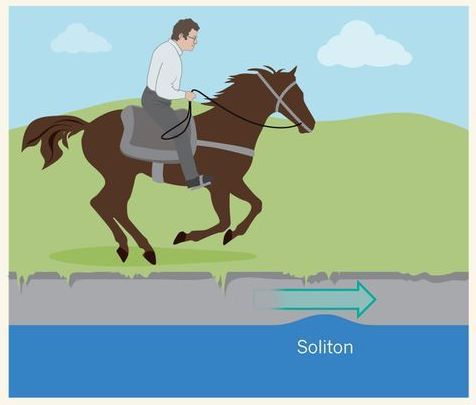
\includegraphics[width=0.6\textwidth]{images/horsebefore.jpg}
\end{figure}
``I followed it on horseback, and overtook it still rolling on at a rate of some eight or nine miles an hour.''
\end{frame}

\begin{frame}
\fontsize{18}{7.2}\selectfont
\begin{figure}[H]
\centering
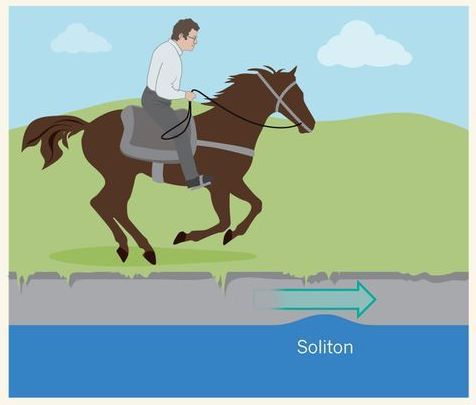
\includegraphics[width=0.6\textwidth]{images/horsebefore.jpg}
\end{figure}
``It continued its course along the channel apparently without change of form or diminution of speed.''
\end{frame}

\begin{frame}
\fontsize{18}{7.2}\selectfont
Russell could create solitary waves in the laboratory
\begin{figure}[H]
\centering
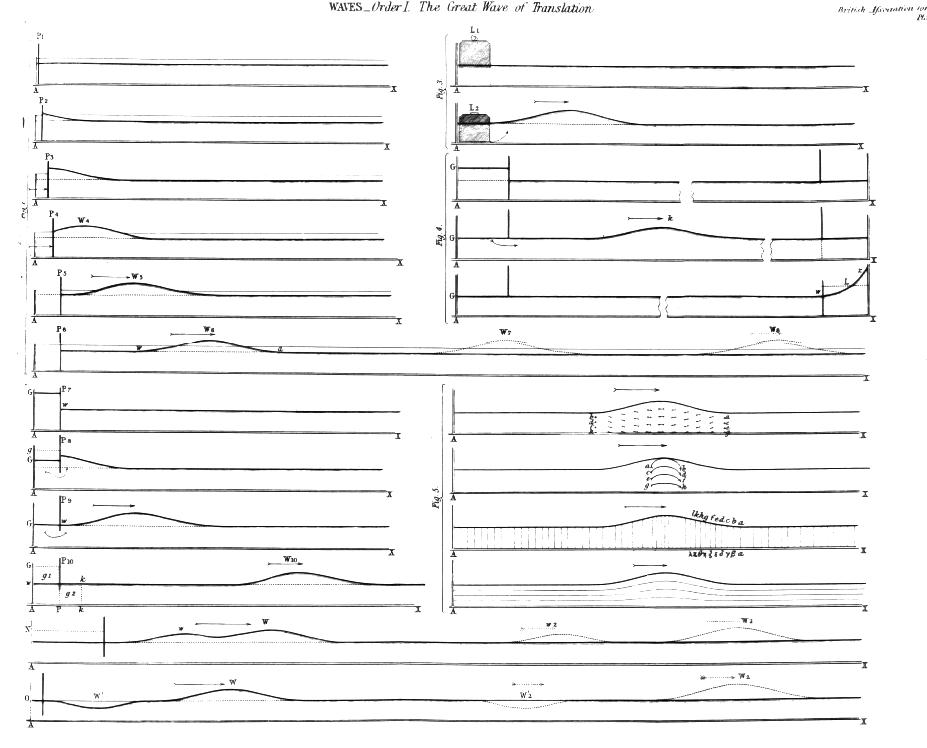
\includegraphics[width=0.6\textwidth]{images/russellwaves.jpg}
\end{figure}
but existing theory could not explain them.
\end{frame}

\begin{frame}
\fontsize{18}{7.2}\selectfont
Solitary wave recreated on the Scott Russell Aqueduct
\begin{figure}[H]
\centering
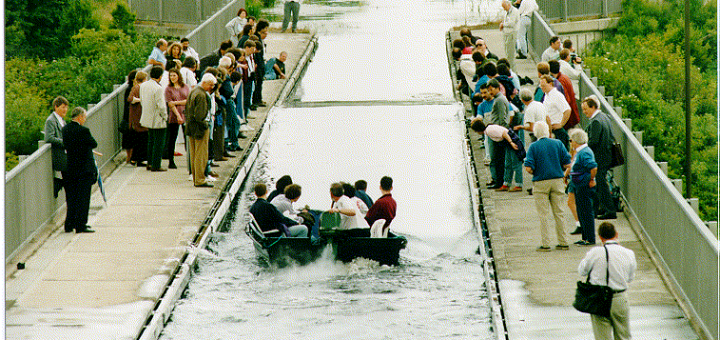
\includegraphics[width=0.8\textwidth]{images/watersoliton.png}
\end{figure}
Department of Mathematics, Heriot-Watt University (1995)
\end{frame}

\begin{frame}
\frametitle{Diederik Korteweg and Gustav de Vries}
\begin{figure}[H]
\centering
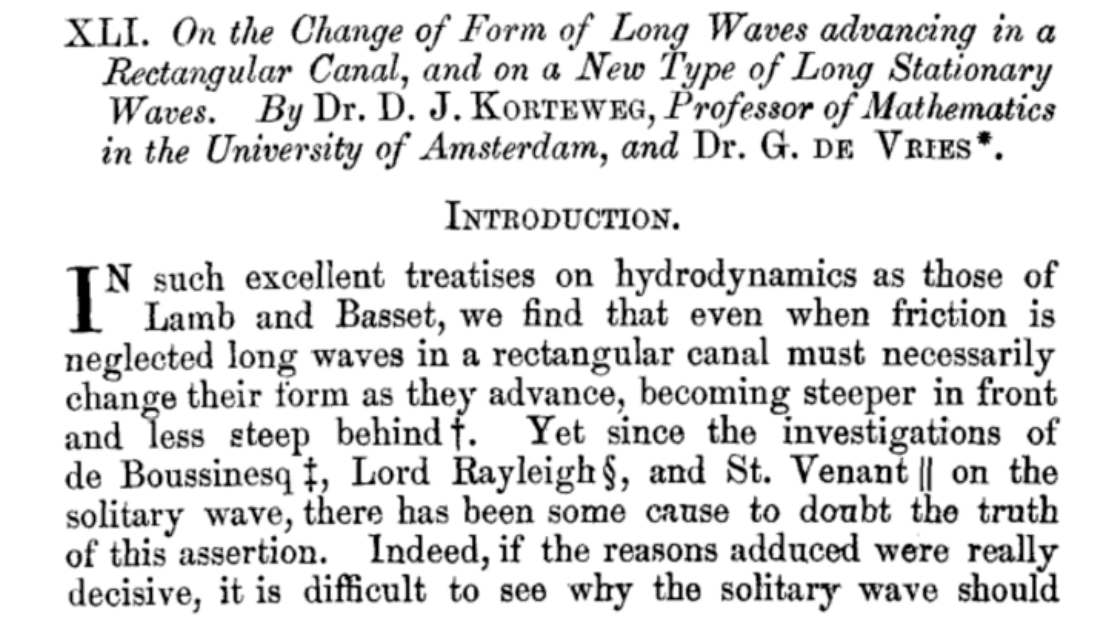
\includegraphics[width=0.6\textwidth]{images/KdVtitle2.png}
\end{figure}
\[
\frac{\partial \eta}{\partial t} = \frac{3}{2} \sqrt{\frac{g}{l}}\cdot
\frac{\partial
\left( \frac{1}{2} \eta^2 + \frac{2}{3} \alpha \eta + \frac{1}{3} \sigma \frac{\partial^2 \eta}{\partial x^2}\right)}{\partial x}
\]
Philosophical Magazine, 1895.
\end{frame}

\begin{frame}
\frametitle{Korteweg-de Vries equation (KdV)}
\fontsize{16}{7.2}\selectfont
Balance between nonlinear advection and dispersion.
\[
u_t + \underbrace{u_{xxx}}_{\text{Dispersion}} - \underbrace{6 u u_x}_{\text{Advection}} 
= 0
\]
\begin{figure}[H]
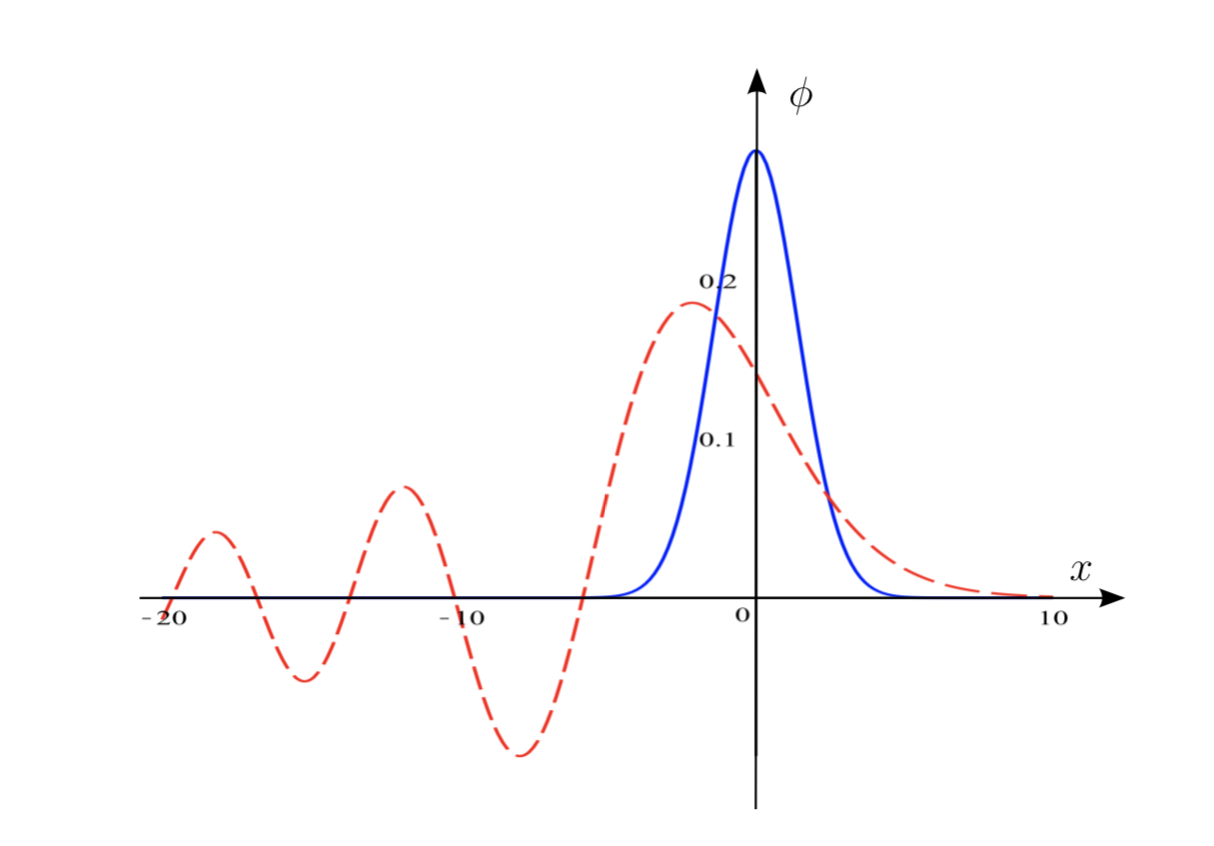
\includegraphics[width=0.45\textwidth]{images/dispersion.png}
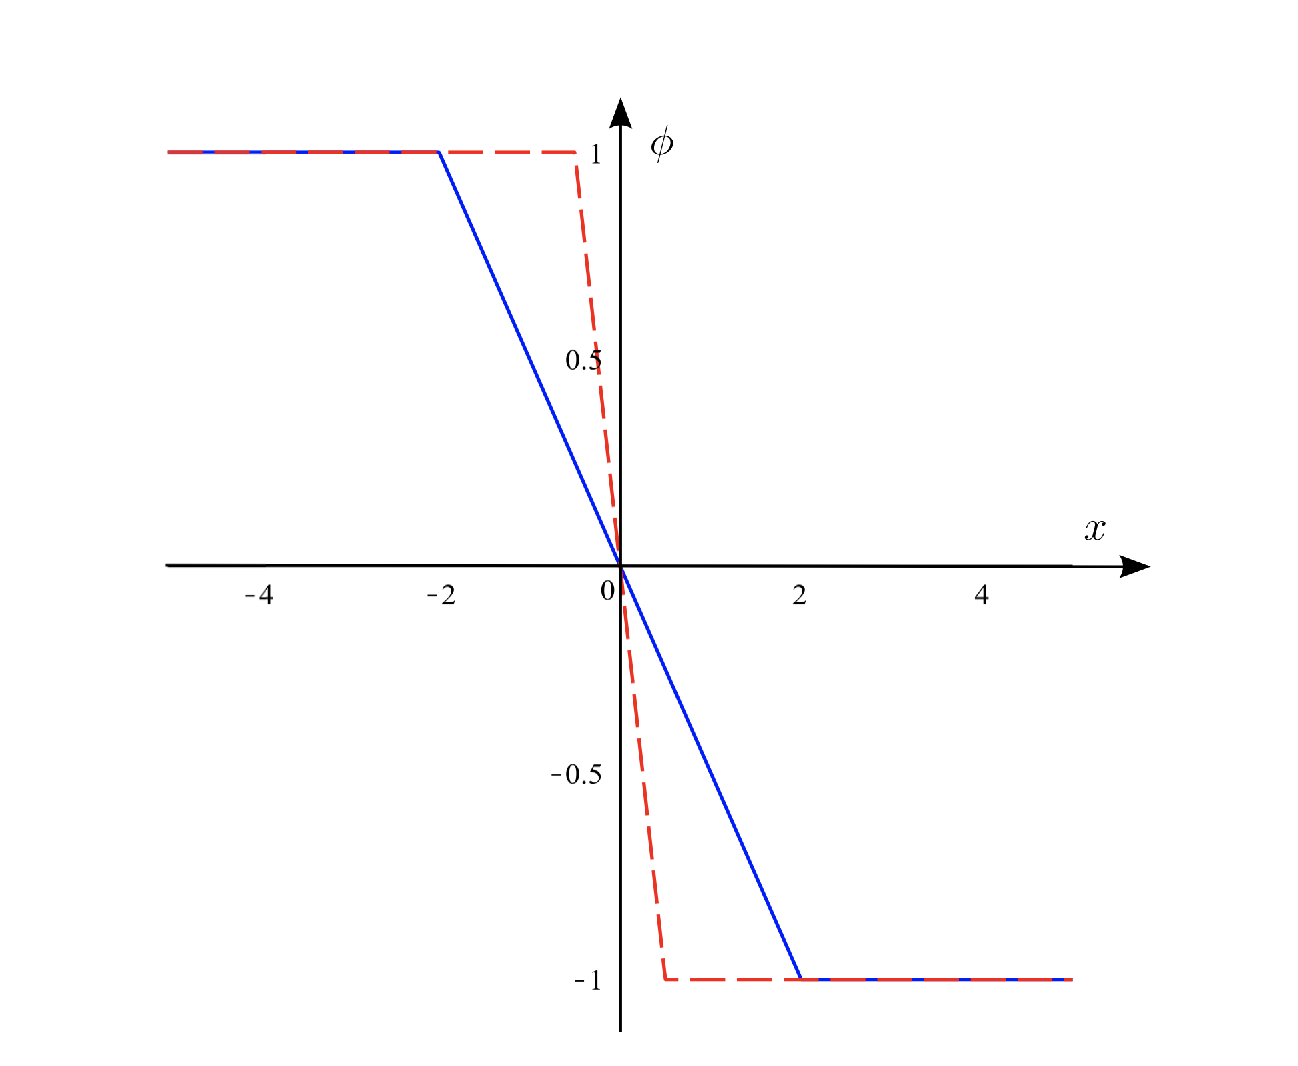
\includegraphics[width=0.45\textwidth]{images/nladvection.png}
\end{figure}
\end{frame}

\begin{frame}
\frametitle{KdV: spatial dynamics}
\fontsize{16}{7.2}\selectfont
Solitary waves with speed $c$ satisfy
\[
u_{xx} - c u - 3 u^2 = 0
\]
Spatial dynamics: write as 1st order ODE
\[
\begin{pmatrix}u \\ v
\end{pmatrix}'
= \begin{pmatrix}
v \\ c u + 3 u^3
\end{pmatrix}
\]
\end{frame}

\begin{frame}
\frametitle{KdV: spatial dynamics}
\fontsize{16}{7.2}\selectfont
\begin{figure}[H]
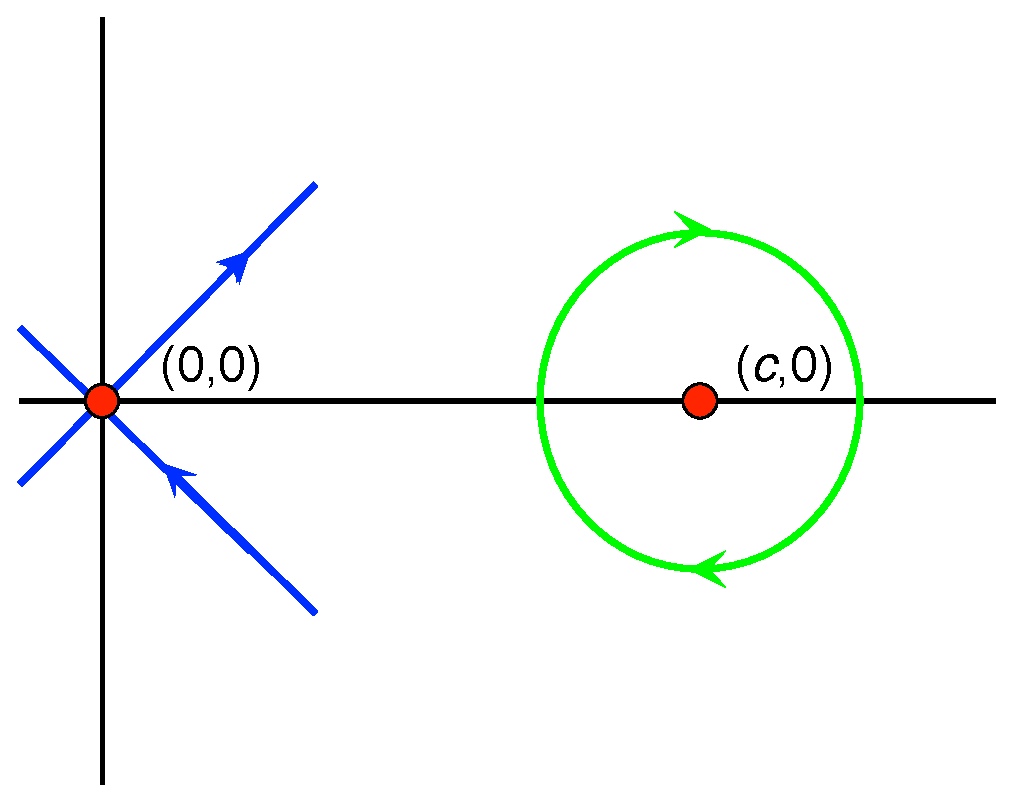
\includegraphics[width=0.6\textwidth]{images/kdv3portrait1.eps}
\end{figure}
\begin{itemize}
\item Saddle node at $(0,0)$: eigenvalues $\pm \sqrt{c}$.
\item Linear center at $(c, 0)$: eigenvalues $\pm \sqrt{c} i$.
\end{itemize}
\end{frame}

\begin{frame}
\frametitle{KdV: solitary waves}
\fontsize{16}{7.2}\selectfont

\begin{figure}[H]
\begin{center}
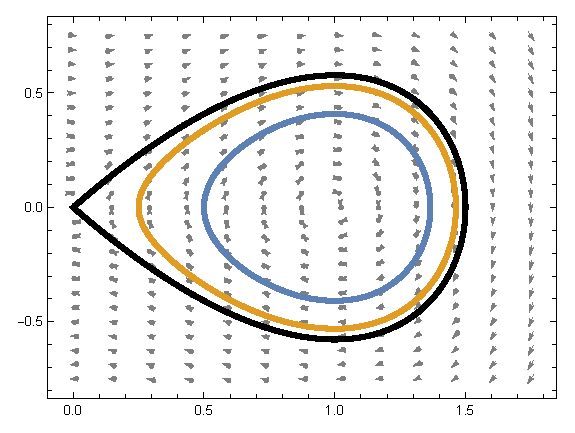
\includegraphics[width=0.4\textwidth]{images/KdV3phaseportrait.eps}
\end{center}
\end{figure}

\begin{figure}[H]
\begin{center}
\begin{tabular}{cc}
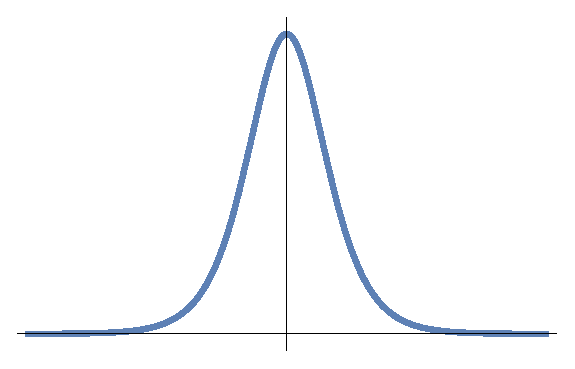
\includegraphics[width=0.4\textwidth]{images/singlepulse.eps} & 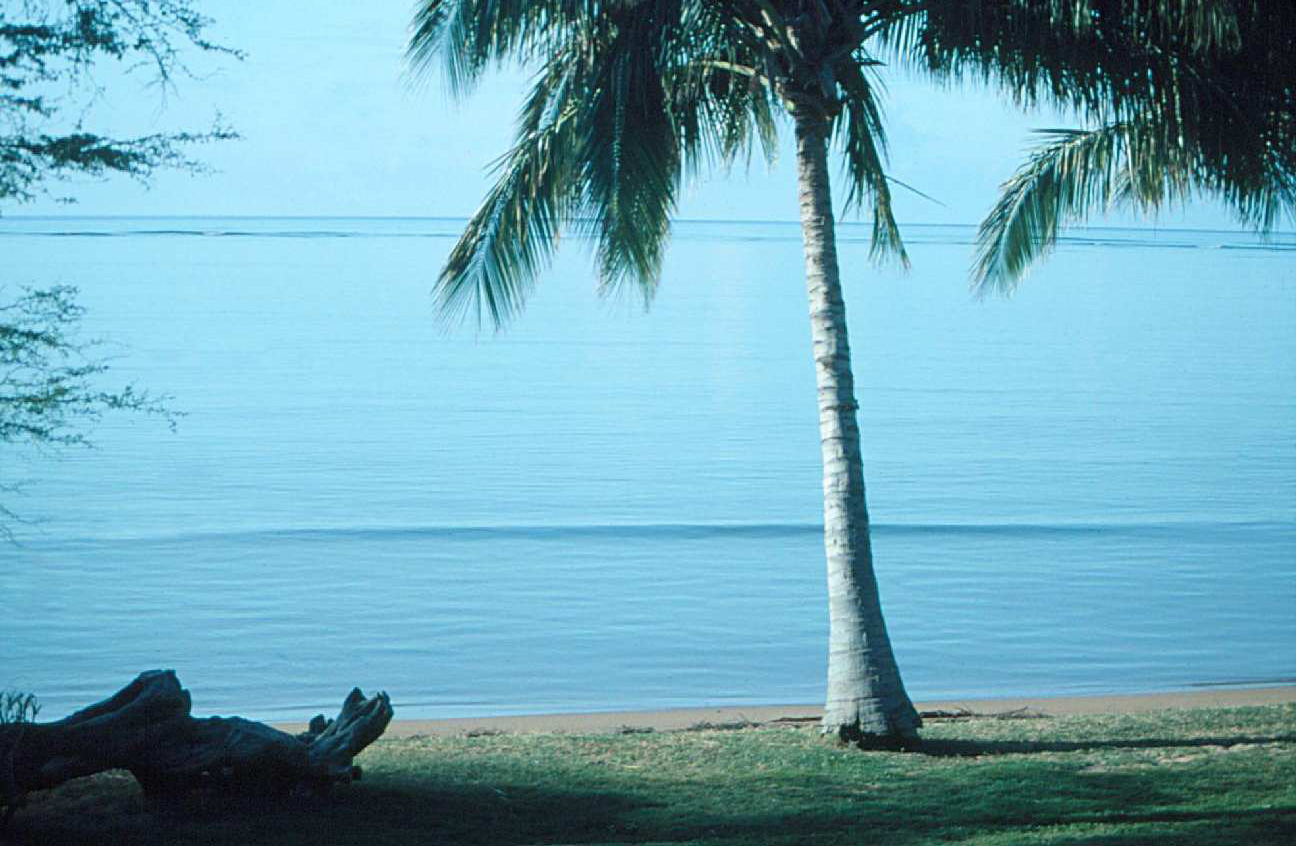
\includegraphics[width=0.4\textwidth]{images/beach.jpg} \\
\end{tabular}
\end{center}
\end{figure}
\end{frame}

\begin{frame}
\frametitle{KdV: periodic waves}
\fontsize{16}{7.2}\selectfont

\begin{figure}[H]
\begin{center}
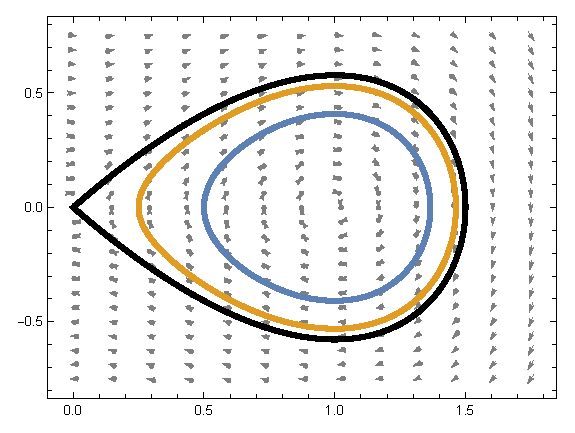
\includegraphics[width=0.4\textwidth]{images/KdV3phaseportrait.eps}
\end{center}
\end{figure}

\begin{figure}[H]
\begin{center}
\begin{tabular}{cc}
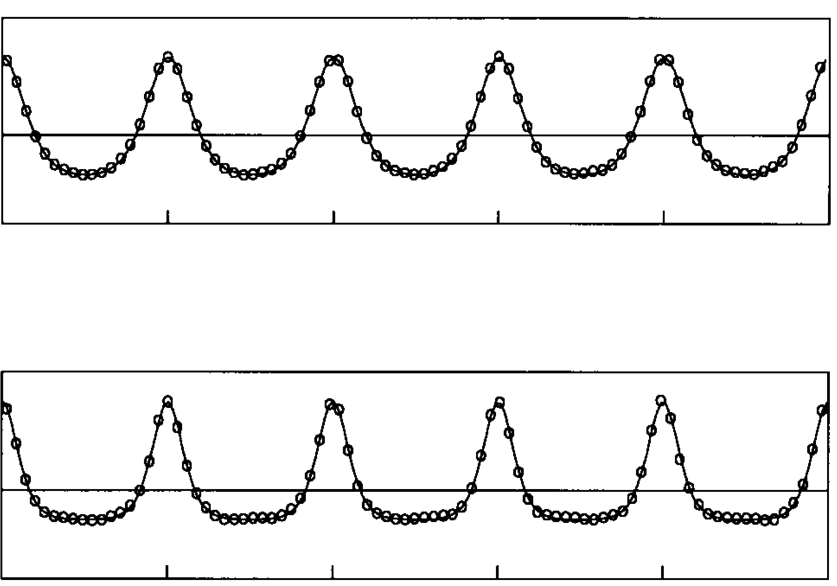
\includegraphics[width=0.4\textwidth]{images/cnoidal3.png} & 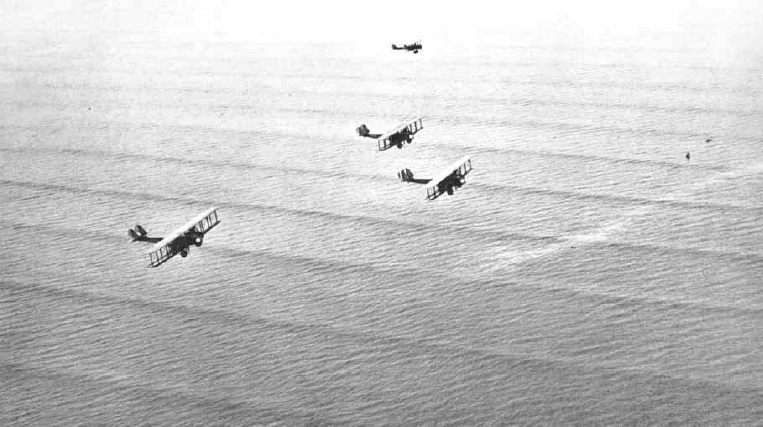
\includegraphics[width=0.4\textwidth]{images/cnoidal.jpg}
\end{tabular}
\end{center}
\end{figure}
\end{frame}

\begin{frame}
\frametitle{KdV: multi-pulses}
\fontsize{16}{7.2}\selectfont

\begin{figure}[H]
\begin{center}
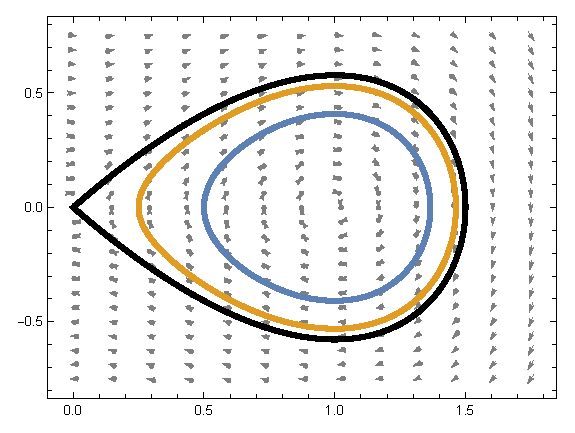
\includegraphics[width=0.4\textwidth]{images/KdV3phaseportrait.eps}
\end{center}
\end{figure}

Multi-pulses are multi-loop homoclinic orbits
\begin{itemize}
	\item Cannot exist in KdV since trajectories in the plane cannot cross
	\item Require spatial dynamics to evolve in a higher dimensional phase space 
\end{itemize}

\end{frame}

\section{Fifth-order KdV equation}

\begin{frame}
	\frametitle{Fifth-order KdV equation (KdV5)}   
	\fontsize{16}{7.2}\selectfont
	\begin{center}
		\[ u_t = u_{xxxxx} - u_{xxx} - 2 u u_x \]
	\end{center}
	\vspace{0.5cm}
	Weakly nonlinear long wave approximation to capillary-gravity wave problem
	\vspace{0.5cm}
	\begin{itemize}
		\item Long wave approximation
		\begin{itemize} 
			\item Wavelength long compared to wave depth
		\end{itemize}
		\item Capillary-gravity waves
		\begin{itemize}
		    \item Influenced by surface tension and gravity
		    \item Longer wavelength than ripples
		    \item Shorter wavelength than ordinary water waves 
		\end{itemize}
		\item Other applications: Plasma waves, laser optics
	\end{itemize}
\end{frame}

\begin{frame}
	\frametitle{Traveling wave solutions}
	\fontsize{16}{7.2}\selectfont
	\begin{itemize}
		\item In co-moving frame with speed $c$
		\begin{center}
		\[ u_t = u_{xxxxx} - u_{xxx} + c u_x - 2 u u_x \]
		\end{center}

		\item Hamiltonian structure
		\begin{center}
		\begin{align*} 
			u_t &= \partial_x E'(u) \\
			E(u) &= -\int_{-\infty}^{\infty} \left( \frac{1}{2}u_{xx}^2 + \frac{1}{2}u_x^2 + \frac{1}{2}cu^2 - \frac{1}{3}u^3 \right) dx 
		\end{align*}
		\end{center}
	\end{itemize}
\end{frame}

\begin{frame}
	\frametitle{Equilibrium solutions}
	\fontsize{16}{7.2}\selectfont
	\begin{itemize}
		\item Equilibrium solutions satisfy 4th order ODE
		\begin{center}
		\[u_{xxxx} - u_{xx} + cu - u^2 = 0\]
		\end{center}
		\vspace{0.25cm}
		\item Eigenvalues of linearization about rest state
		\begin{center}
		\includegraphics[width=0.7\textwidth]{images/eigbifurcation2}
		\end{center}
		For $c > 1/4$, quartet $\pm \alpha \pm \beta i$
	\end{itemize}
\end{frame}

\begin{frame}
	\frametitle{Homoclinic orbits}
	\fontsize{16}{7.2}\selectfont

	Symmetric homoclinic orbits exist for $c > 0$ \\ \footnotesize [Groves (1998), Chugunova and Pelinovsky (2007)]

	\begin{figure}
   		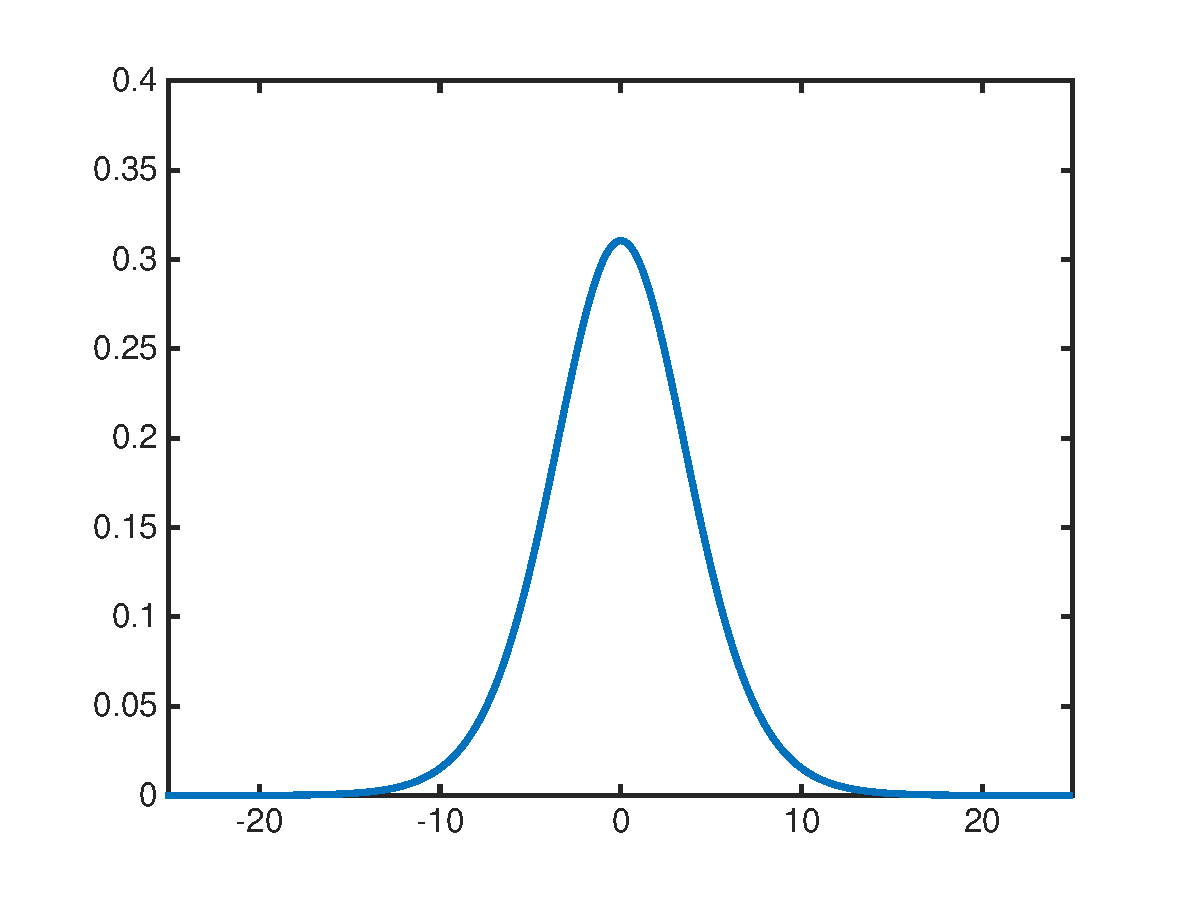
\includegraphics[width=0.48\textwidth]{images/exactsol}
   		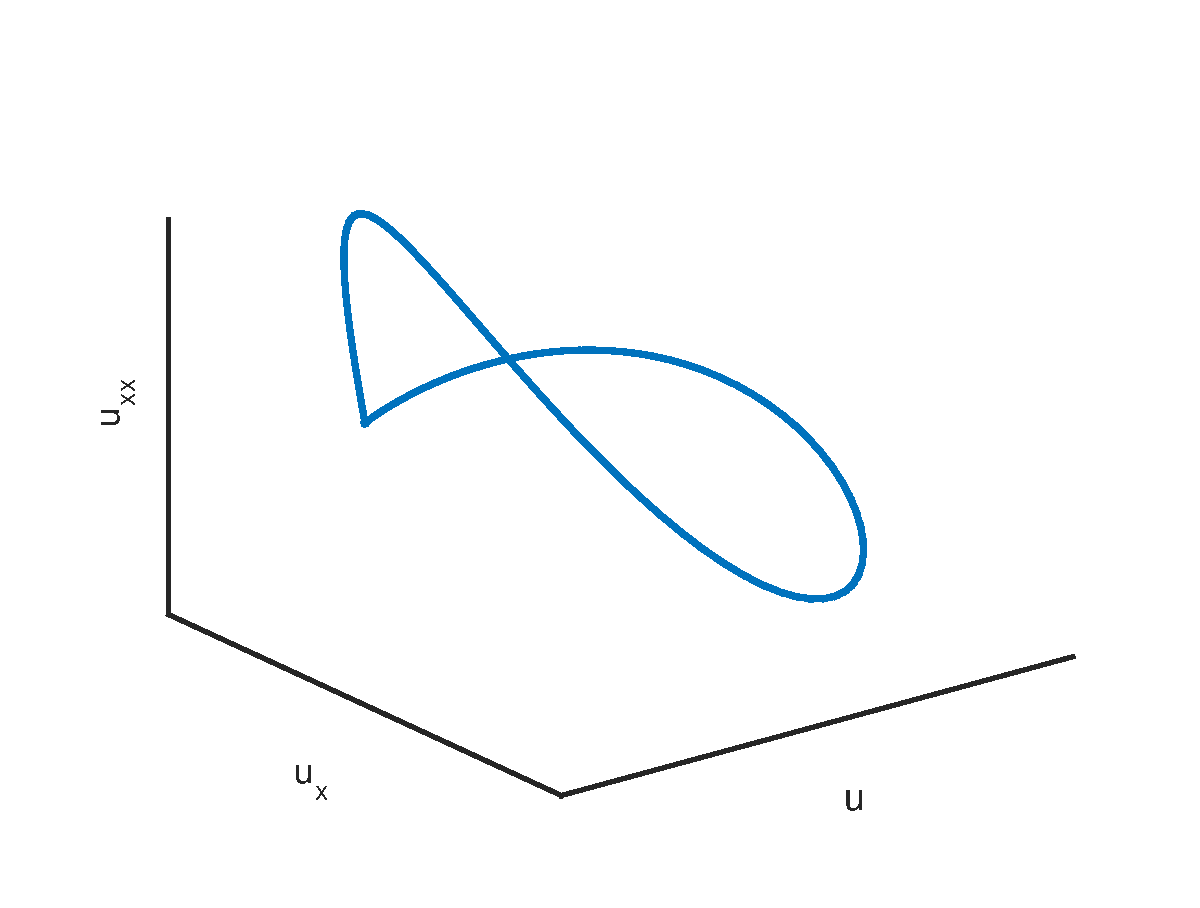
\includegraphics[width=0.48\textwidth]{images/exactsolorbit}
	\end{figure}
\end{frame}

\begin{frame}
\frametitle{Multi-pulse solutions} 
	\fontsize{16}{7.2}\selectfont
    \begin{block}{Theorem [Buffoni et al. (1996); Sandstede (1997)]}
    For $c > 1/4$, multi-pulse solutions exist, which resemble copies of the primary pulse spliced together.

	\begin{figure}
	\begin{center}
	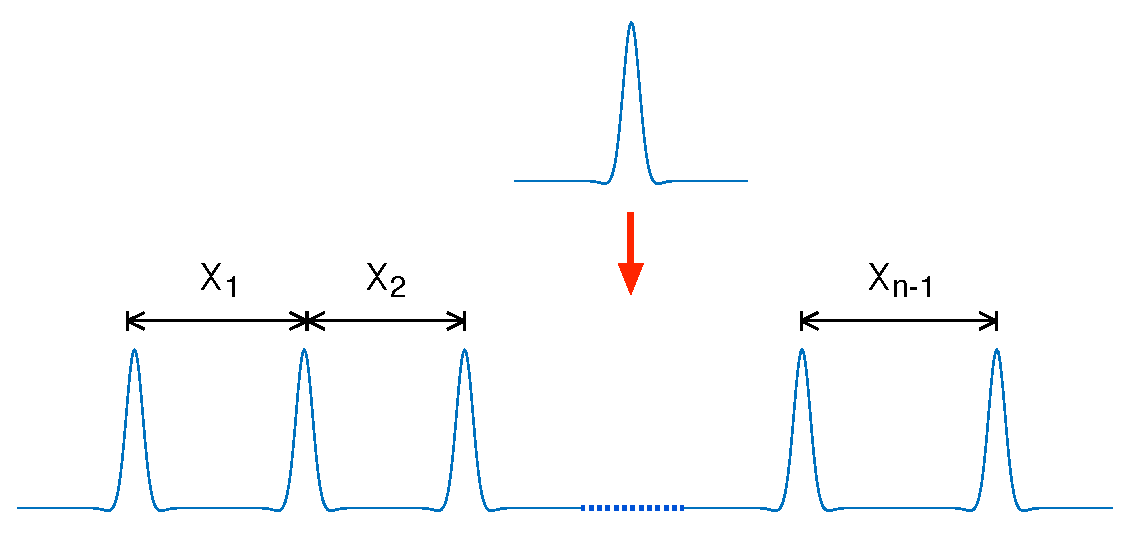
\includegraphics[width=8cm]{images/multipulse.eps}
	\end{center}
	\begin{align*}
	 X_j &\approx \frac{2 \pi}{\beta} k_j + C && k_j \text{ integer}
	\end{align*}
	\end{figure}

    \end{block}
\end{frame}

\begin{frame}
	\frametitle{Double pulse solutions}
	\fontsize{16}{7.2}\selectfont
	\begin{figure}
	\begin{center}
	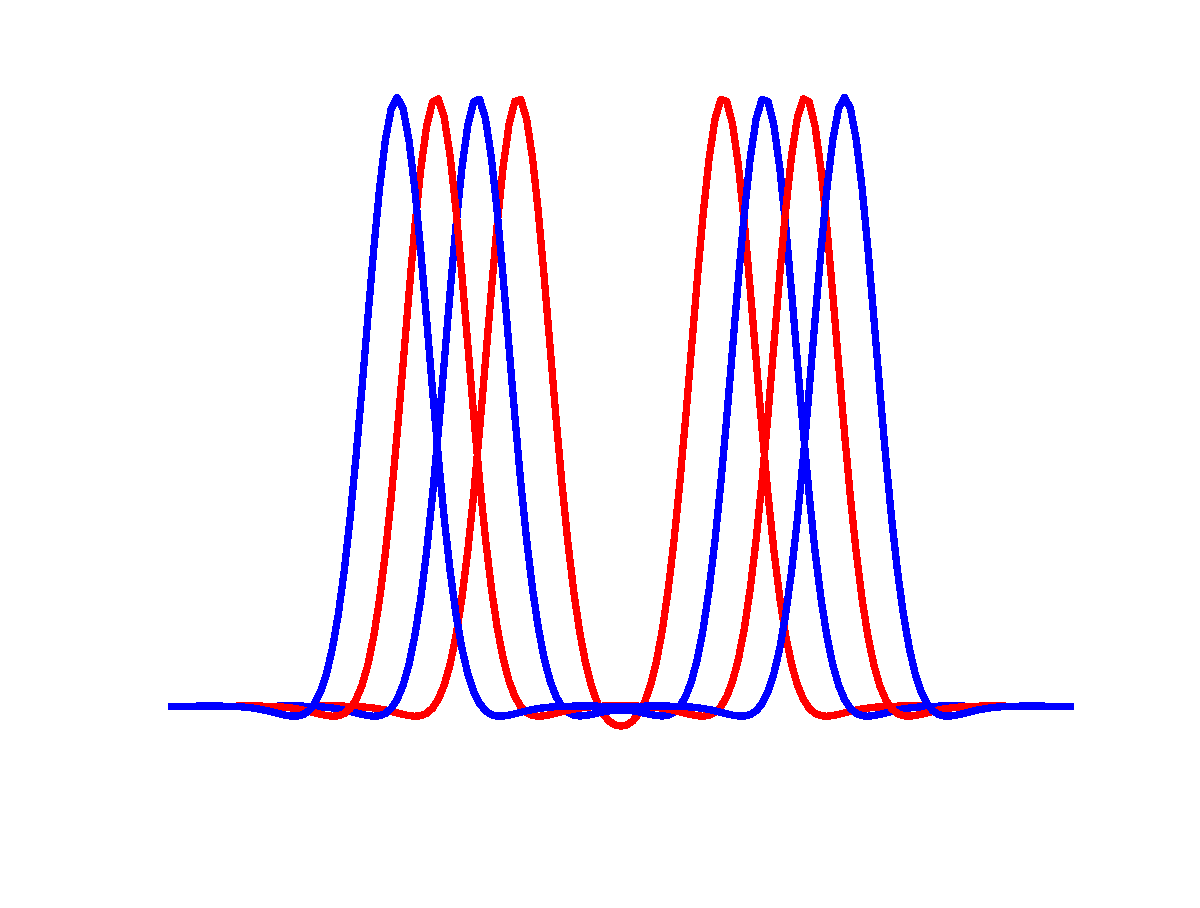
\includegraphics[width=0.7\linewidth]{images/first4dp}
	\end{center}
	\caption{First four double pulses ($c = 10$). \textcolor{red}{$k$ odd}. \textcolor{blue}{$k$ even. } }
	\end{figure}
\end{frame}

\begin{frame}
	\frametitle{Construction of double pulses}
	\fontsize{16}{7.2}\selectfont
	\begin{figure}
	\begin{center}
	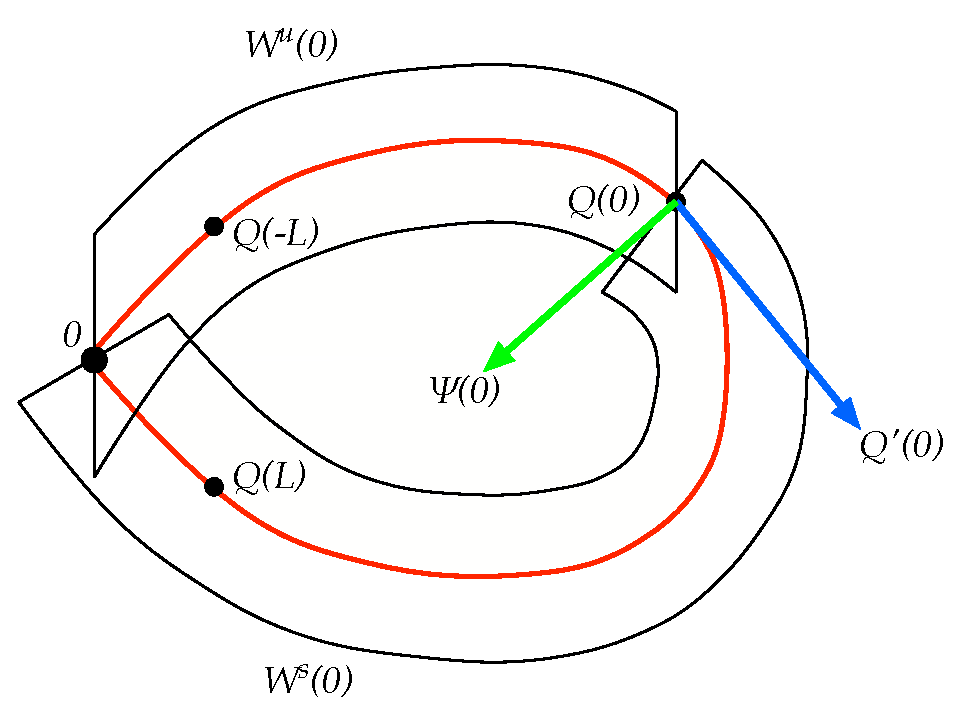
\includegraphics[width=0.6\linewidth]{images/WsWu}
	\end{center}
	\end{figure}
	\begin{itemize}
		\item Homoclinic orbit $Q(x)$ lies in intersection of unstable and stable manifolds
		\item $\Psi(x)$ is perpendicular to both manifolds
	\end{itemize}
\end{frame}

\begin{frame}
	\frametitle{Construction of double pulses}
	\fontsize{16}{7.2}\selectfont
	\begin{figure}
	\begin{center}
	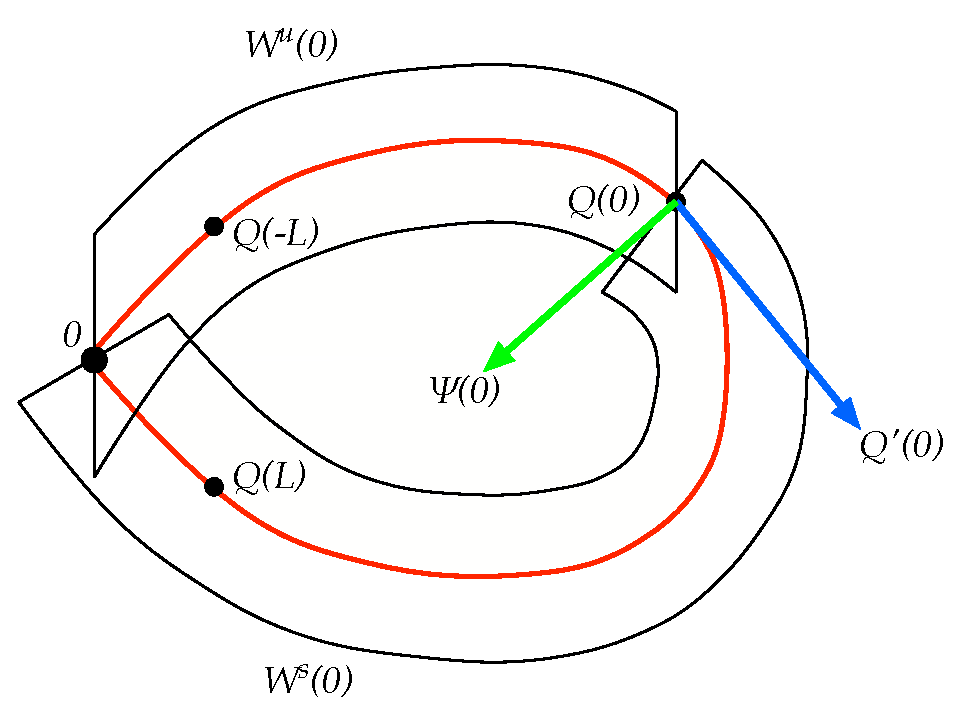
\includegraphics[width=0.6\linewidth]{images/WsWu}
	\end{center}
	\end{figure}
	Double pulse must ``jump'' from stable manifold at $x = L$ to unstable manifold at $ = -L$.
\end{frame}

\begin{frame}
	\frametitle{Construction of double pulses}
	\fontsize{16}{7.2}\selectfont
	For $c > 0$, eigenvalues of rest state are $\pm \alpha \pm \beta i$
	\begin{figure}
	\begin{center}
	\includegraphics[width=0.3\linewidth]{images/eigbifurcationdouble.pdf}
	\end{center}
	\end{figure}
	Stable and unstable manifolds ``twist'' with frequency $\beta$ as they approach the origin
\end{frame}

\begin{frame}
	\frametitle{Construction of double pulses}
	\fontsize{16}{7.2}\selectfont
	\begin{figure}
	\begin{center}
	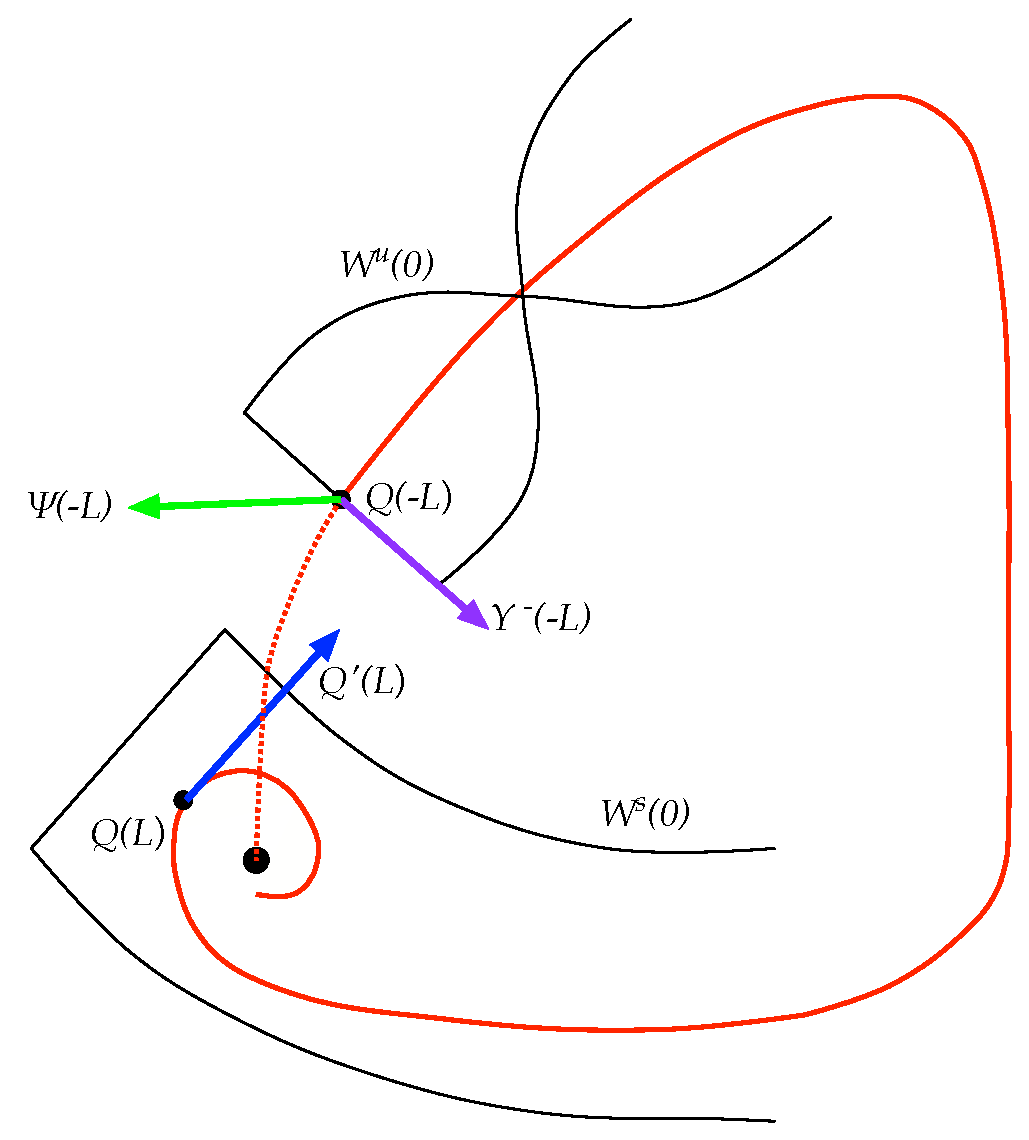
\includegraphics[width=0.45\linewidth]{images/manifoldslineup}
	\end{center}
	\end{figure}
	Specific geometry needed to ``jump'' from stable to unstable manifold: $Q'(L)$ parallel to $\Psi(-L)$.
\end{frame}

\begin{frame}
	\frametitle{Construction of double pulses}
	\fontsize{16}{7.2}\selectfont
	$Q'(x)$ and $\Psi(-x)$ rotate in opposite directions.
	\begin{figure}
	\begin{center}
	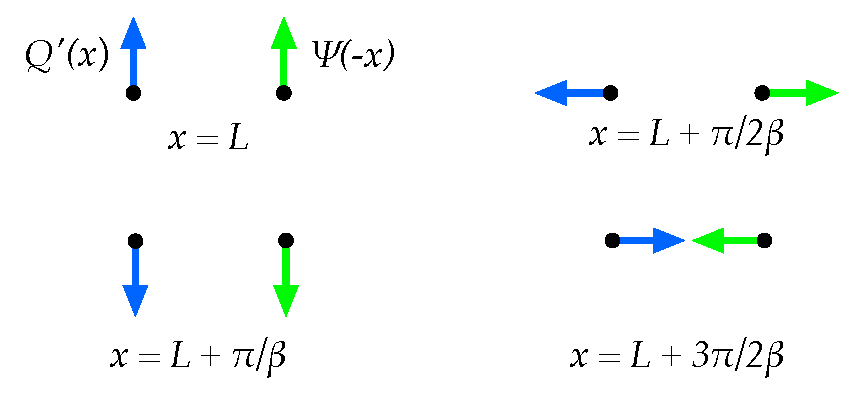
\includegraphics[width=0.6\linewidth]{images/psiqoneperiod} 
	\end{center}
	\end{figure}
	Proper alignment for ``jump'' occurs every quarter period.
\end{frame}

\begin{frame}
	\frametitle{Construction of double pulses}
	\fontsize{16}{7.2}\selectfont
	\begin{figure}
	\begin{center}
	\includegraphics[width=0.6\linewidth]{images/WsWudouble}
	\end{center}
	\end{figure}
\end{frame}

\section{Eigenvalue problem for multi-pulses}

\begin{frame}
	\frametitle{Eigenvalue problem}
	\fontsize{16}{7.2}\selectfont
	Linearization of the PDE about an equilibrium solution $u^*(x)$

	\begin{center}
		$(L - \lambda I )v = 0$
	\end{center}

	\begin{center}
		$L = \partial_x^5 - \partial_x^3 + (c - 2 u^*)\partial_x - 2 u^*_x $
	\end{center}
	Eigenvalues of background state
	\begin{center}
		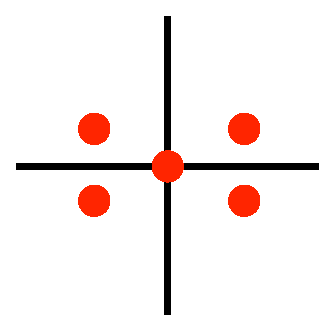
\includegraphics[width=0.2\linewidth]{images/eignonhyp.eps}
	\end{center}
\end{frame}

\begin{frame}
	\frametitle{Spectral theory}
	\fontsize{16}{7.2}\selectfont
	Definitions:
	\begin{itemize}
		\item Resolvent set: $L - \lambda I$ is invertible with bounded inverse
		\vspace{0.5cm}
		\item Spectrum: complement of resolvent set
	\end{itemize}
	\vspace{1cm}
	For our operator $L$:
	\begin{itemize}
		\item Essential spectrum: $L - \lambda I$ is not Fredholm
		\vspace{0.5cm}
		\item Point spectrum (eigenvalues): kernel of $L - \lambda I$ contains an eigenfunction 
	\end{itemize}
\end{frame}

\begin{frame}
	\frametitle{Essential spectrum}
	\fontsize{16}{7.2}\selectfont
	\begin{itemize}
		\item Essential spectrum is entire imaginary axis
			\begin{center}
			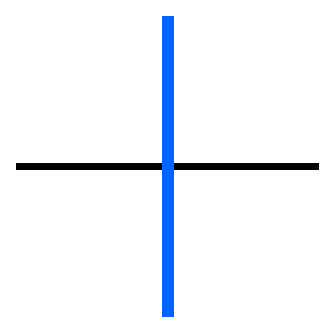
\includegraphics[width=0.3\linewidth]{images/essspec1.eps}
			\end{center}

		\item Depends only on background state.
		\vspace{0.5cm}
		\item Independent of solution we are linearizing about.
	\end{itemize}
\end{frame}

\begin{frame}
	\frametitle{Point spectrum}
	\fontsize{16}{7.2}\selectfont
	\begin{itemize}
		\item Always have double eigenvalue at 0
		\begin{center}
			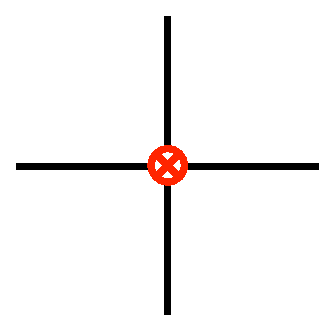
\includegraphics[width=0.3\linewidth]{images/eigsingle.eps}
		\end{center}
		\item From translation invariance
		\vspace{0.5cm}
		\item Eigenfunctions are $\partial_x u^*$ and $\partial_c u^*$
	\end{itemize}
\end{frame}

\begin{frame}
	\frametitle{Spectrum of multi-pulses}
	\fontsize{16}{7.2}\selectfont
	\begin{itemize}
	\item Spectrum of primary pulse
		\begin{center}
			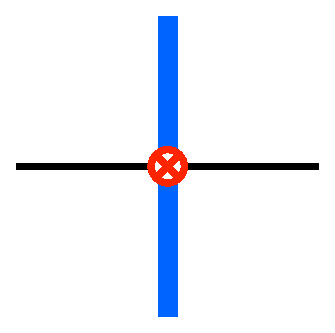
\includegraphics[width=0.2\linewidth]{images/eigsinglepulse.eps}
		\end{center}
	\item For multi-pulses, additional eigenvalues near 0 from interaction between neighboring pulses 
	\fontsize{16}{7.2}\selectfont
	\item Interaction eigenvalues must come in quartets since Hamiltonian system
		\begin{center}
			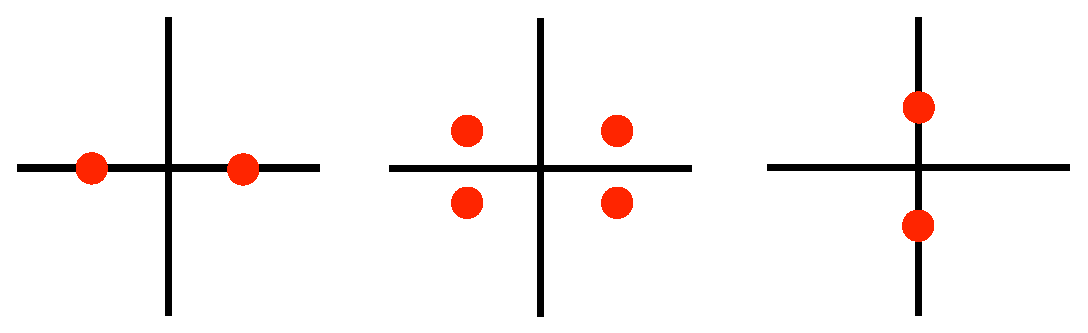
\includegraphics[width=0.8\linewidth]{images/eigdouble2}
		\end{center}
	\end{itemize}
\end{frame}

\begin{frame}
	\frametitle{Spectrum of double pulses}
	\begin{center}
		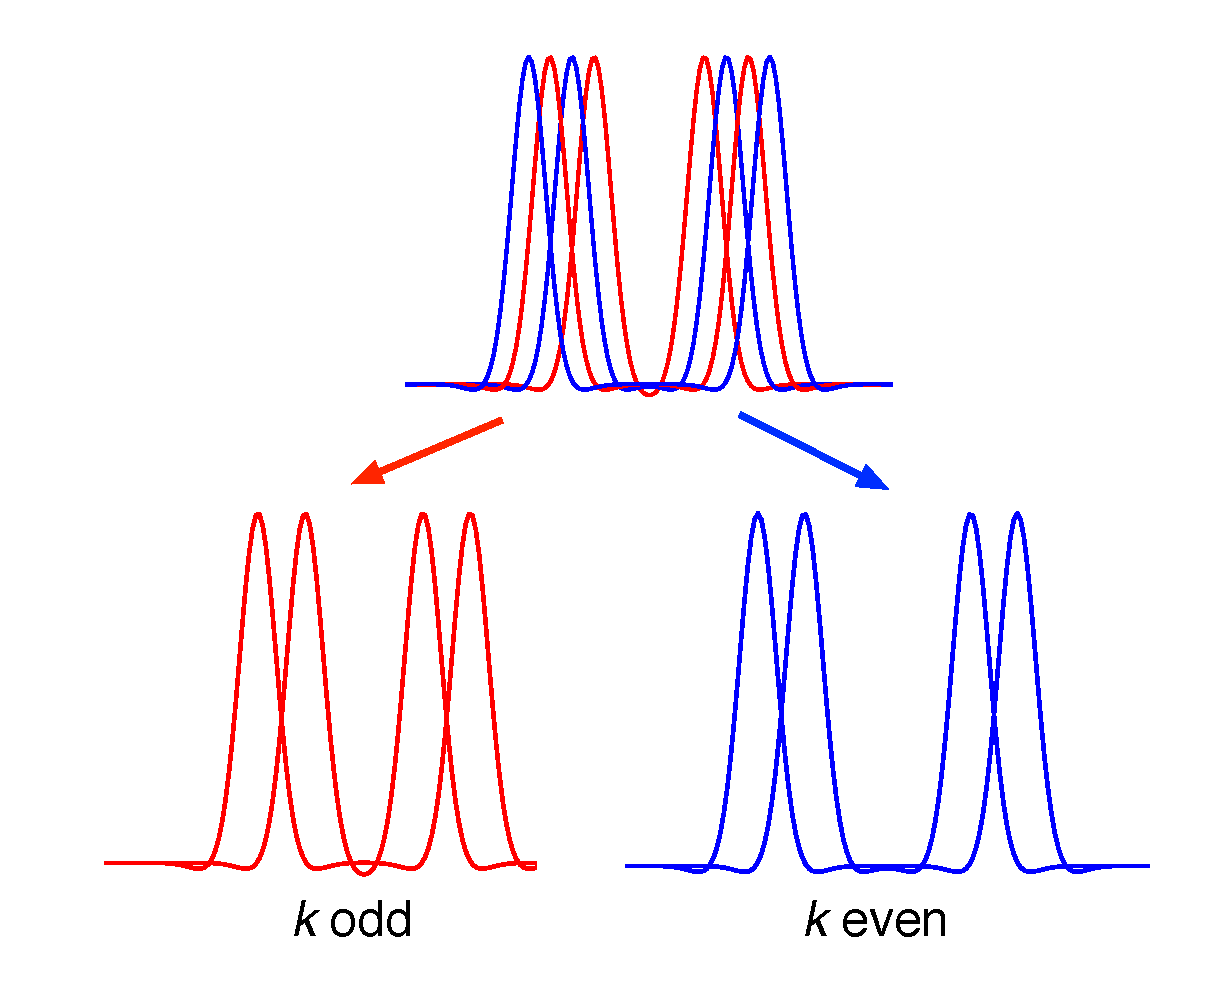
\includegraphics[width=0.8\linewidth]{images/dpsplit}
	\end{center}
\end{frame}

\begin{frame}
	\frametitle{Unstable double pulses ($k$ odd)}
	\fontsize{16}{7.2}\selectfont
	\begin{center}
		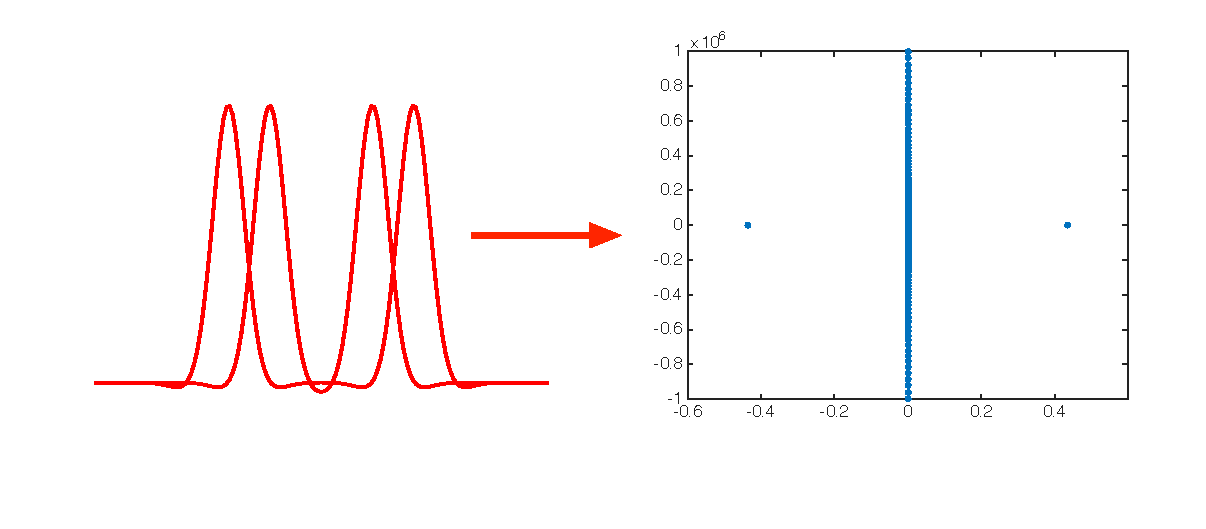
\includegraphics[width=1\linewidth]{images/doubleunstableeig}
	\end{center}
	\begin{itemize}
	\item Pair of real interaction eigenvalues.
	\item Can prove this occurs.
	\end{itemize}
\end{frame}

\begin{frame}{Neutrally stable double pulses ($k$ even)}
	\fontsize{16}{7.2}\selectfont
	\begin{center}
		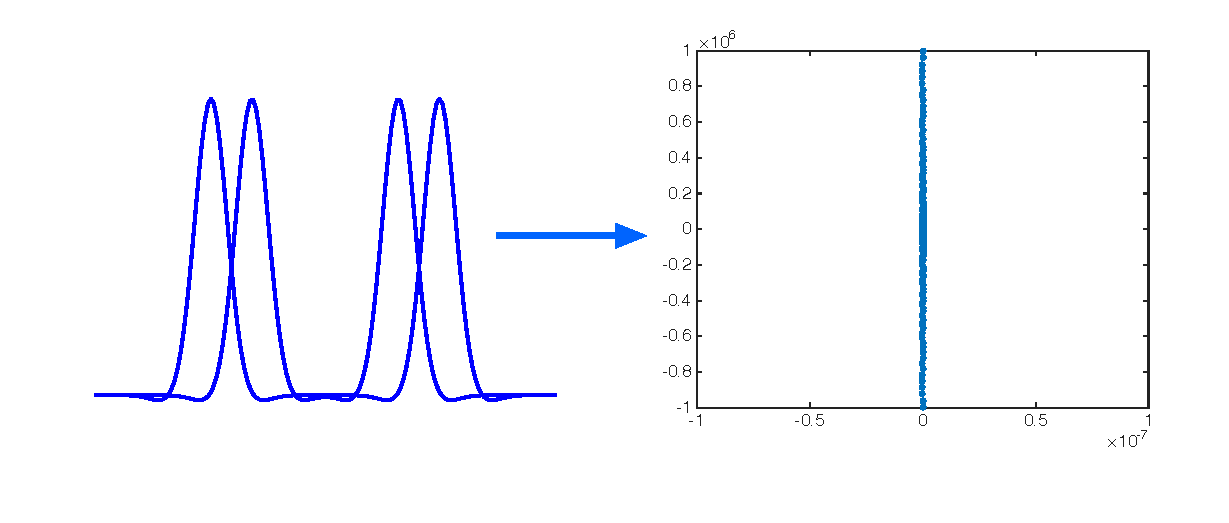
\includegraphics[width=1\linewidth]{images/doublestableeig}
	\end{center}
	\begin{itemize}
	\item Where are the interaction eigenvalues?
	\item If they are embedded in the essential spectrum, how would you locate them?
	\end{itemize}
\end{frame}

\begin{frame}{Neutrally stable double pulses}
	\fontsize{14}{7.2}\selectfont
	\begin{center}
		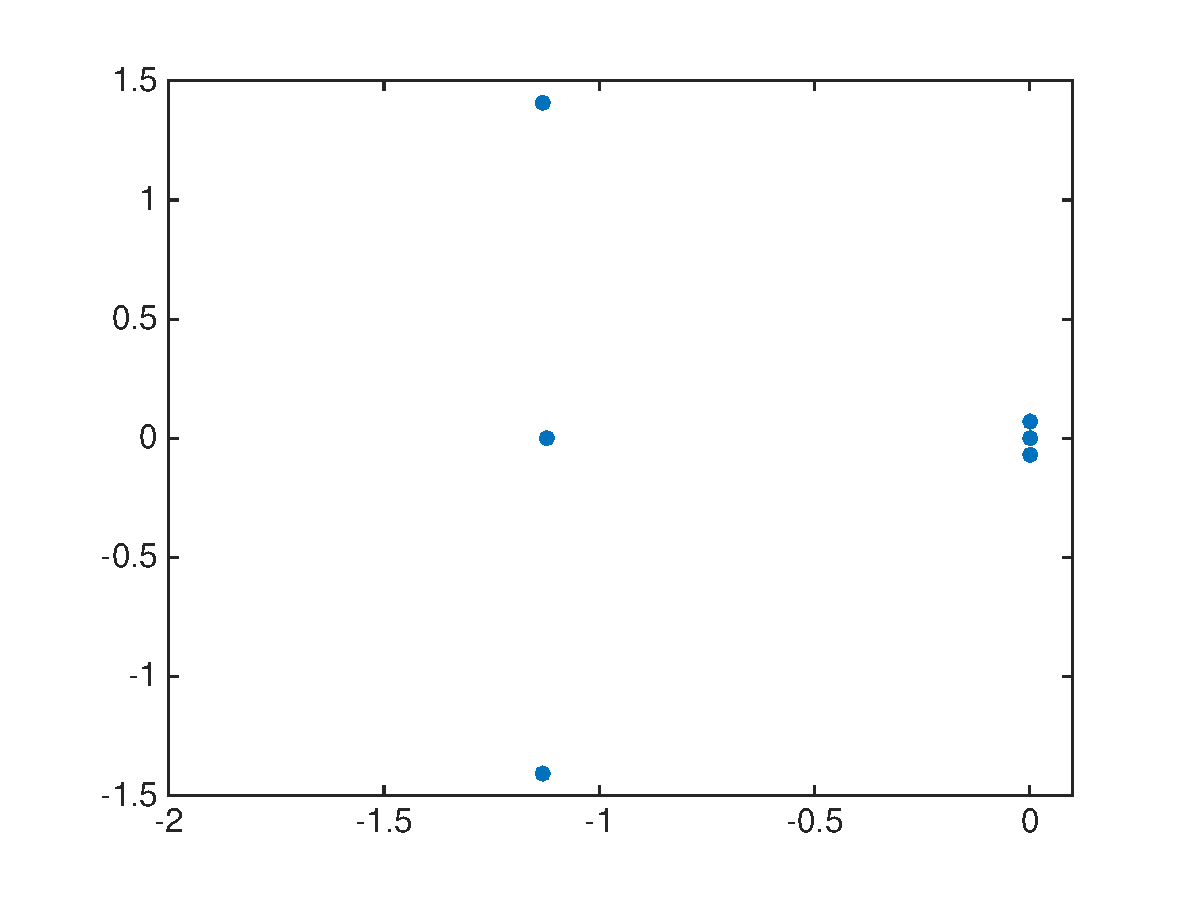
\includegraphics[width=0.5\linewidth]{images/stableeigweighted2}
	\end{center}
	\begin{itemize}
		\item Exponential weight shifts essential spectrum to left
		\item System no longer Hamiltonian with exponential weight
		\item Can only prove interaction eigenvalues are pure imaginary to leading order 
	\end{itemize}
\end{frame}

\section{Periodic multi-pulses}

\begin{frame}
	\frametitle{Periodic multi-pulses}
	\fontsize{16}{7.2}\selectfont
	\begin{itemize}
		\item Essential spectrum becomes discrete
		\vspace{0.5cm}
		\item We don't have to look for embedded eigenvalues
		\vspace{0.5cm}
		\item Each pulse interacts with its two neighbors
		\vspace{0.5cm}
		\item This interaction constrains the allowable pulse distances
		\vspace{0.5cm}
		\item Essential spectrum eigenvalues and interaction eigenvalues can collide
	\end{itemize}
\end{frame}

\begin{frame}
\frametitle{Periodic multi-pulses} 
	\fontsize{14}{7.2}\selectfont
    \begin{block}{Theorem [P.]}
    For sufficiently large $X_j$, periodic multi-pulse solutions exist\footnote{Some restrictions apply.}.

	\begin{figure}
	\begin{center}
	\includegraphics[width=8cm]{images/multipulseperiodic2.pdf}
	\end{center}
	\end{figure}
    \end{block}
\end{frame}

\begin{frame}
\frametitle{Periodic multi-pulses} 
	\fontsize{14}{7.2}\selectfont
    \begin{block}{Theorem [P.]}
    2-periodic pulses with $X_0 \neq X_1$ bifurcate from 2-periodic pulses with $X_0 = X_1$ in a series of pitchforks.

	\begin{figure}
	\begin{center}
	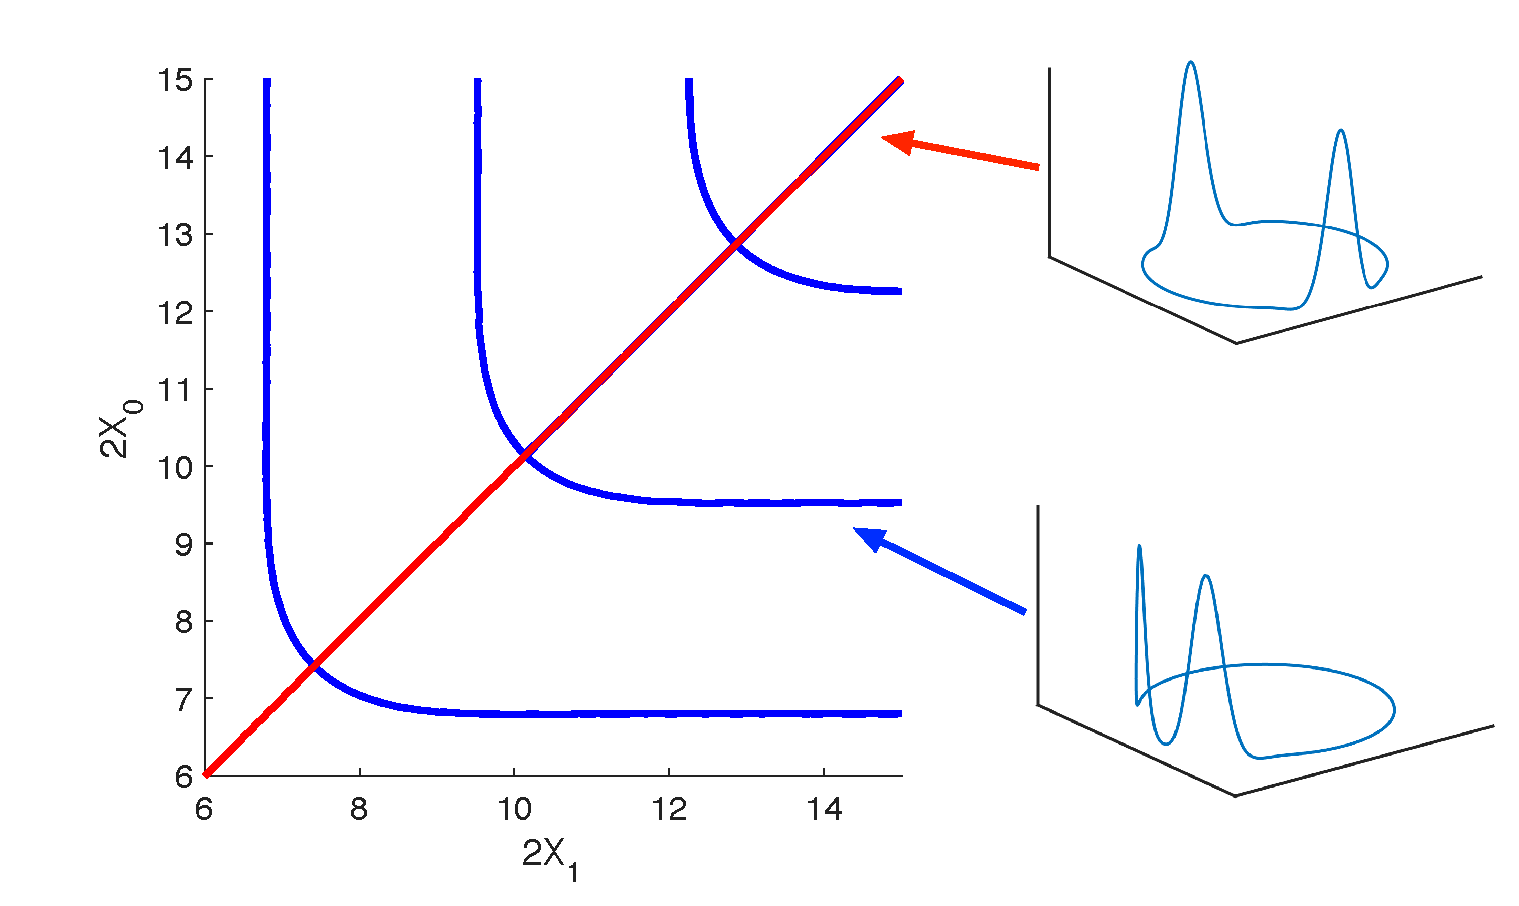
\includegraphics[width=7.25cm]{images/periodicpitchforklabeled}
	\end{center}
	\end{figure}
    \end{block}
\end{frame}

\begin{frame}
	\frametitle{Location of eigenvalues}
	\fontsize{16}{7.2}\selectfont
	We expect to find two categories of eigenvalues.

	\begin{itemize}
		\item Discrete ``essential spectrum'' eigenvalues along the imaginary axis.
		\begin{itemize}
			\item Depend only on background state and domain size
			\item Independent of solution we linearize about
		\end{itemize}
		\item Eigenvalues resulting from pulse interaction 
		\begin{itemize}
			\item Each pulse interacts with two neighbors
			\item Depend on geometry of periodic multi-pulse
		\end{itemize}
	\end{itemize}
	\vspace{0.5cm}

	By Hamiltonian symmetry, eigenvalues must come in quartets.
\end{frame}

\begin{frame}
	\frametitle{Location of eigenvalues}
	\fontsize{16}{7.2}\selectfont
	Idea: Construct eigenfunctions as linear combinations of the kernel eigenfunction $\partial_x q(x)$
	\begin{figure}
	\begin{center}
	\begin{tabular}{cc}
	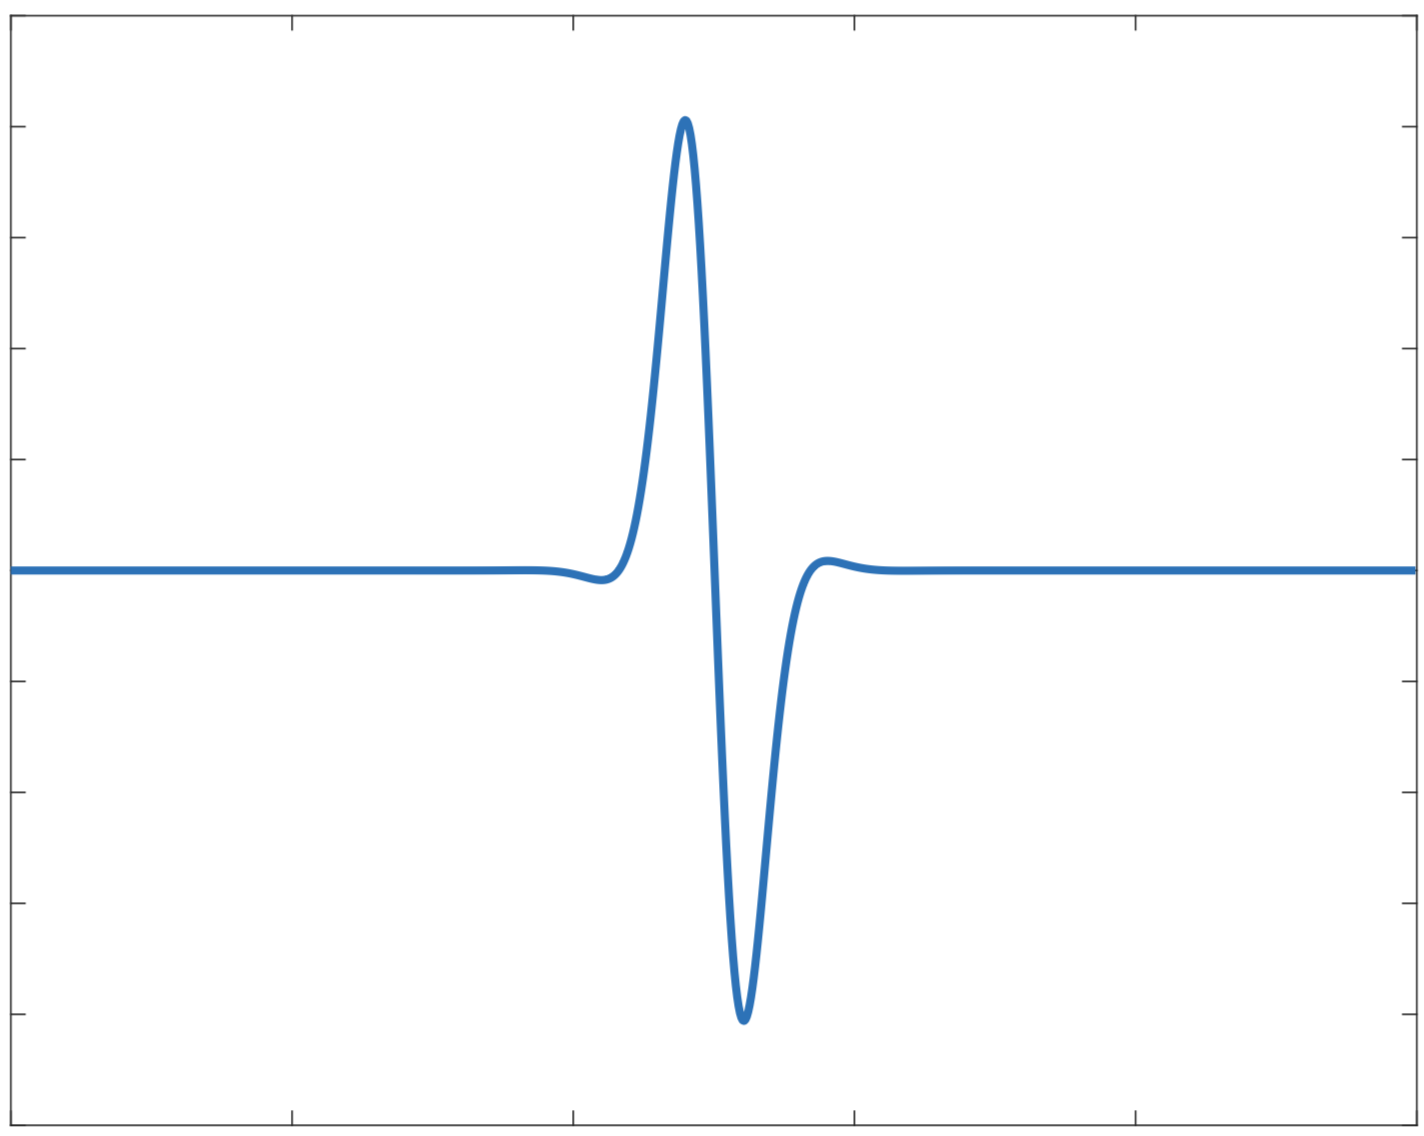
\includegraphics[width=0.4\textwidth]{images/kerneleig} & 
	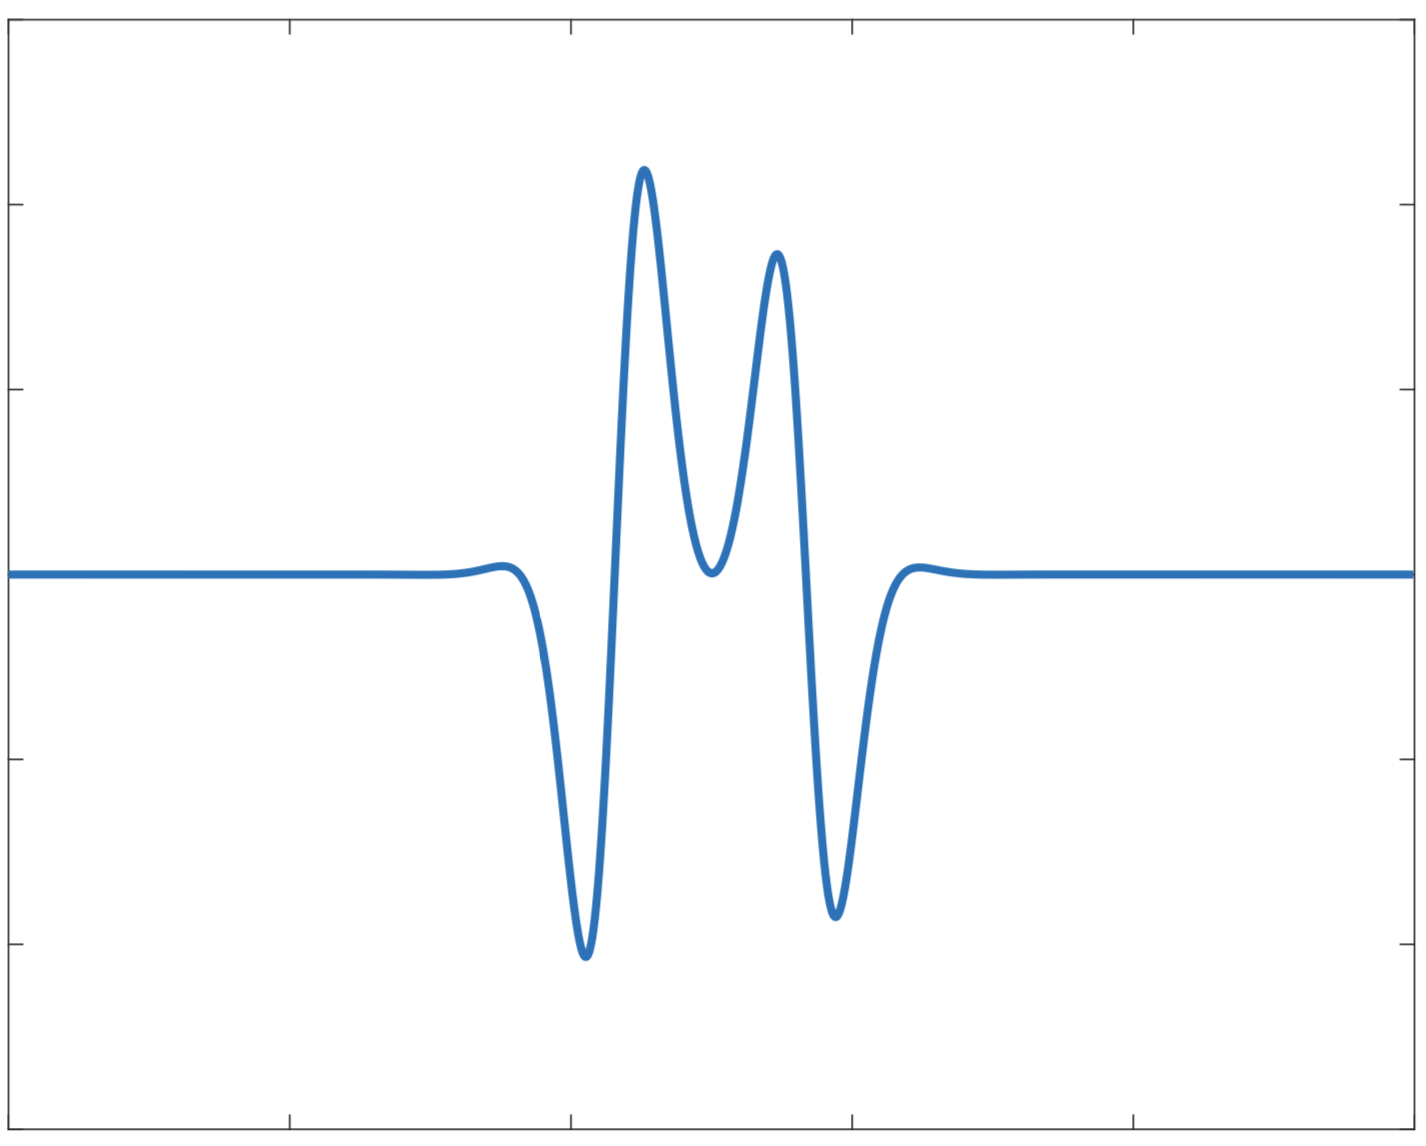
\includegraphics[width=0.4\textwidth]{images/DP1eig} \\
	\end{tabular}
	\end{center}
	\end{figure}
	Reduces eigenvalue problem to finding determinant of a matrix.
\end{frame}

\begin{frame}
\frametitle{Location of eigenvalues} 
	\fontsize{14}{7.2}\selectfont
    \begin{block}{Theorem [P.]}
    $\lambda$ is a PDE eigenvalue for the linearization about a periodic $n-$pulse on $[-X, X]$ if and only if 
    \[
    \det\begin{pmatrix}
K(\lambda) + C_1 & \lambda K_2(\lambda) - \lambda^2 \tilde{M}^c I + D_1 \\
-\frac{1}{2} \lambda M^c K_1(\lambda) + C_2 & A - \lambda^2 MI + D_2
\end{pmatrix} = 0
    \]
    \begin{itemize}
    	\item $K(\lambda)$ is an $n \times n$ matrix which depends only on the background state
    	\item $A$ is an $n \times n$ matrix which depends on the geometry of the $n$-pulse
    	\item $M$, $M^c$, and $\tilde{M}^c$ are constants.
    	\item The rest are higher order terms.
    \end{itemize}
    \end{block}
\end{frame}

\begin{frame}
\frametitle{Location of eigenvalues} 
	\fontsize{14}{7.2}\selectfont
    \begin{block}{Theorem (simpler)}
    $\lambda$ is a PDE eigenvalue for the linearization about a periodic $n-$pulse on $[-X, X]$ if and only if 
    \[
    \det\begin{pmatrix}K(\lambda) & 0 \\ 0 & A - \lambda^2  M I \end{pmatrix} + \text{``h.o.t.''} = 0
    \]
    The higher order terms decay exponentially in the pulse distances $X_j$.
    \end{block}
\end{frame}

\begin{frame}
\frametitle{Location of eigenvalues} 
	\fontsize{14}{7.2}\selectfont
    \begin{block}{Theorem [P. ]}
    For a periodic 2-pulse on $[-X, X]$, as long as
    \begin{itemize}
    	\item We are not at the pitchfork bifurcation point
    	\item The period is not ``too large''
    \end{itemize}
    We have
    \begin{itemize}
    	\item An eigenvalue with algebraic multiplicity 3 at 0
    	\item A pair of interaction eigenvalues which are either real or imaginary.
    	\item Discrete pairs of imaginary essential spectrum eigenvalues located at
    	\begin{align*}
    	\lambda_m^{\text{ess}}(r) &\approx c \frac{m \pi i}{X} && m \text{ nonzero integer}
    	\end{align*}
    \end{itemize}
    \end{block}
\end{frame}

\begin{frame}
\frametitle{Location of eigenvalues} 
	\fontsize{14}{7.2}\selectfont
    \begin{block}{Theorem [P. ]}
    For a periodic 2-pulse, as long as the period is not ``too large'', we have the following interaction eigenvalue pattern
    	\begin{figure}
		\begin{center}
		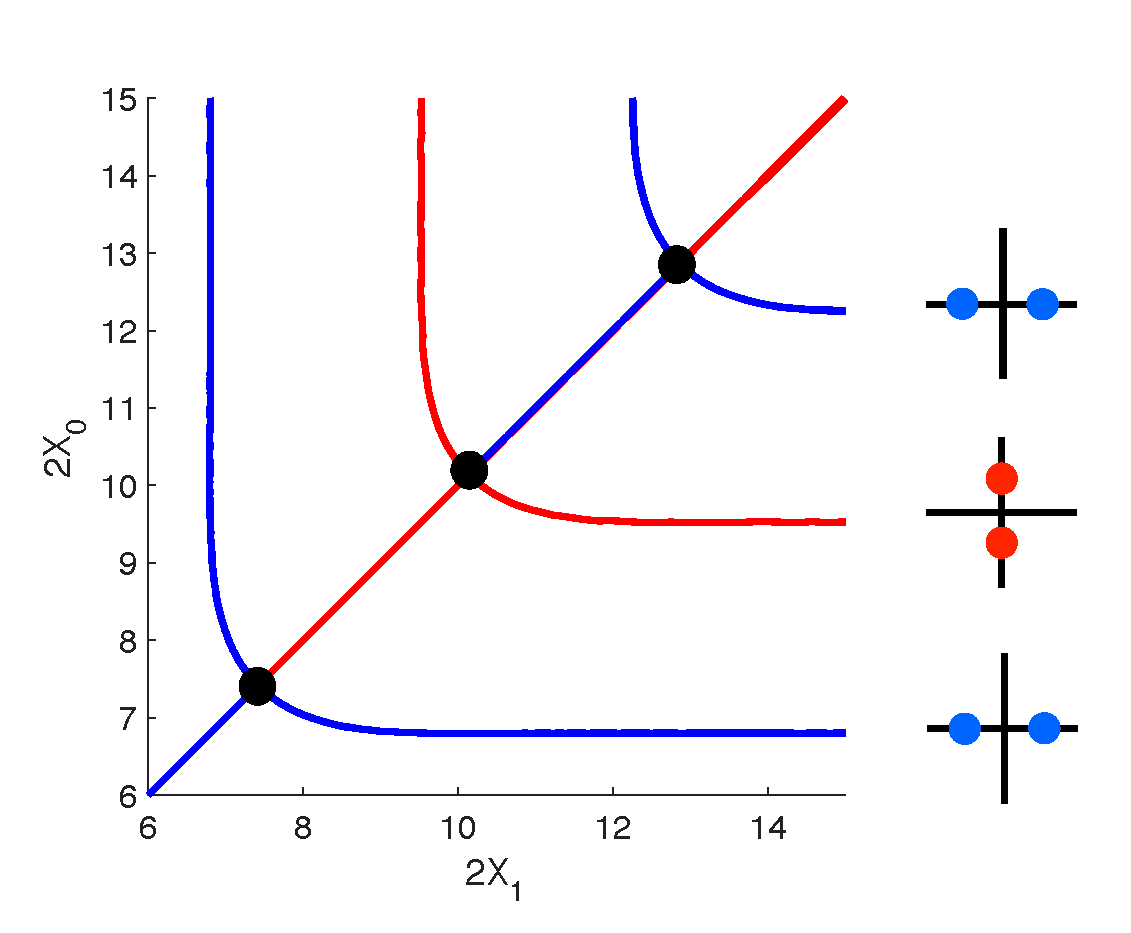
\includegraphics[width=7cm]{images/2periodiceigpattern.eps}
		\end{center}
		\end{figure}
    \end{block}
\end{frame}

\begin{frame}
	\frametitle{Location of eigenvalues}
	\fontsize{16}{7.2}\selectfont
		\begin{figure}
		\begin{center}
		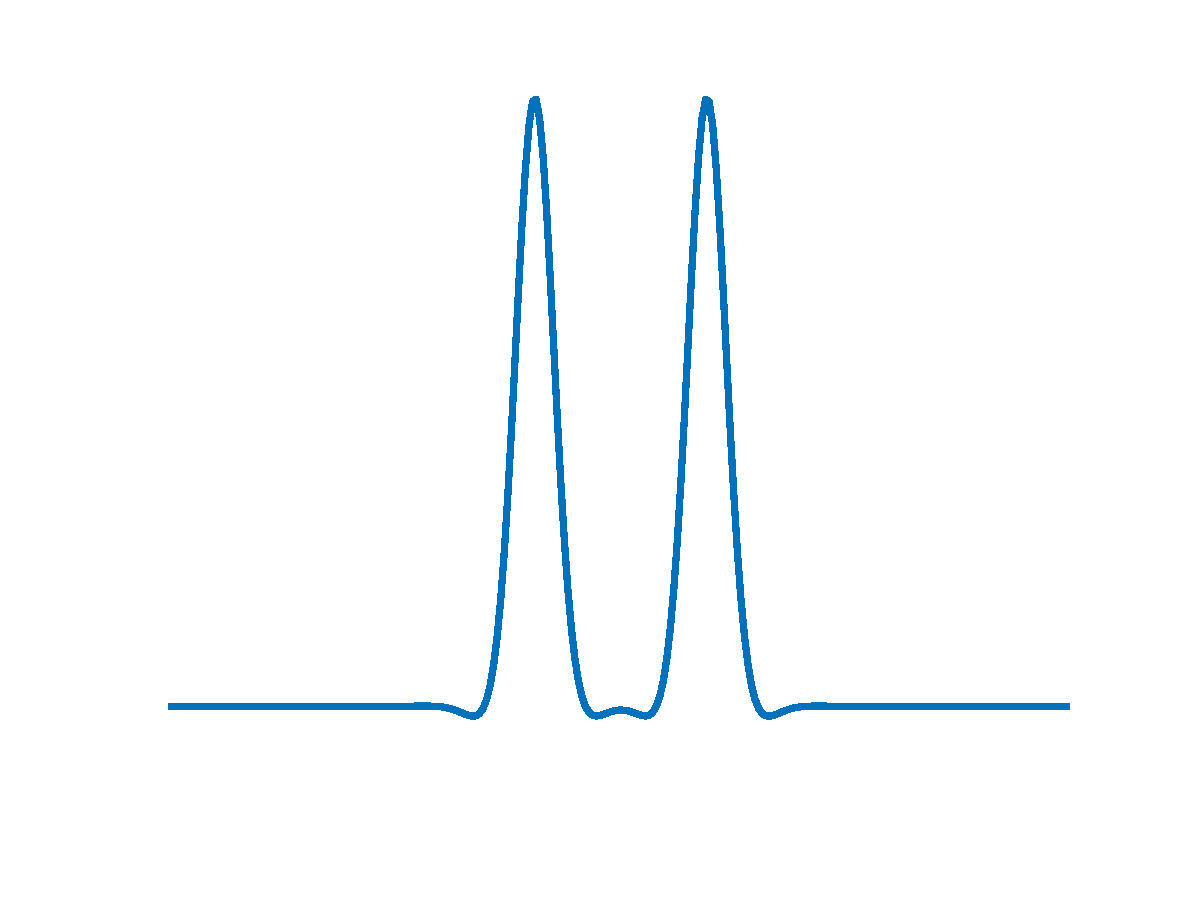
\includegraphics[width=4cm]{images/2pulsestable}
		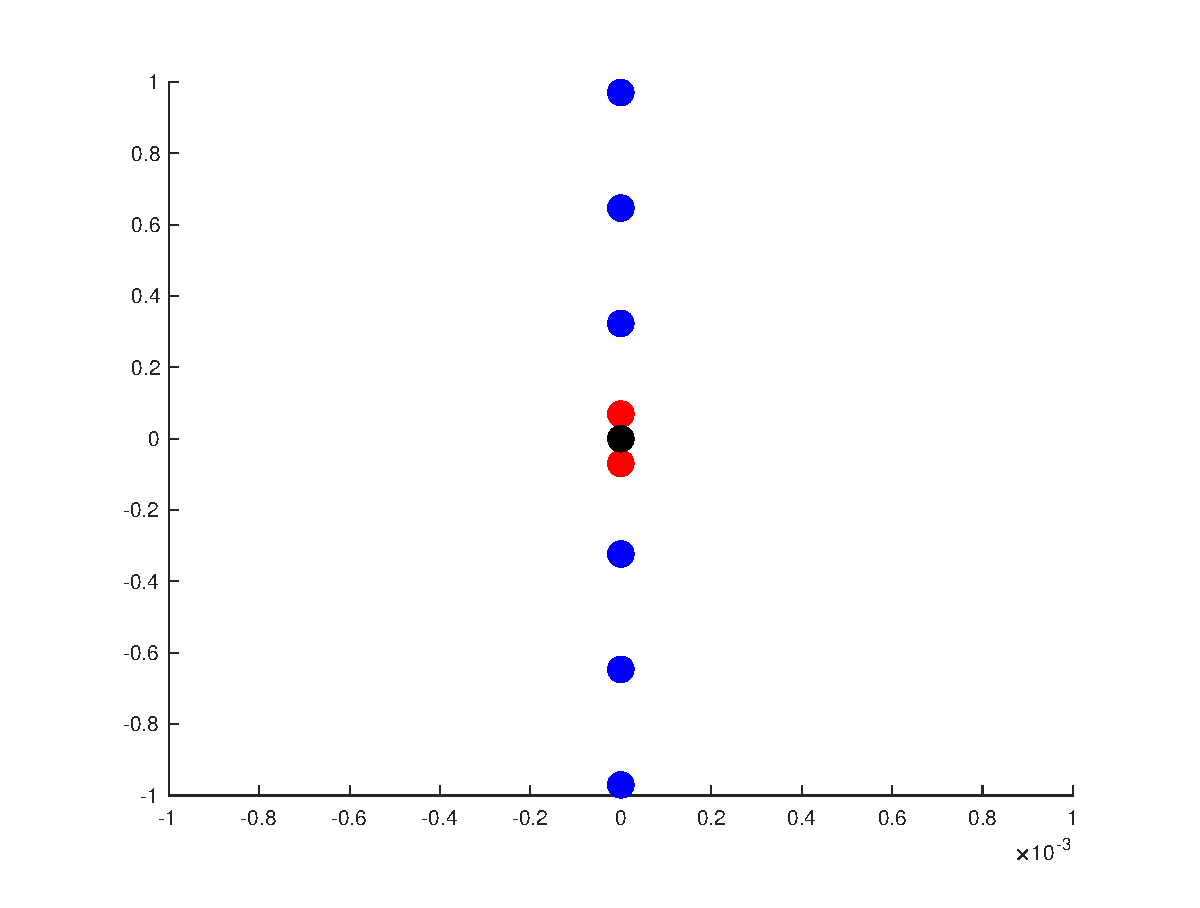
\includegraphics[width=4cm]{images/2pulsestableeig}
		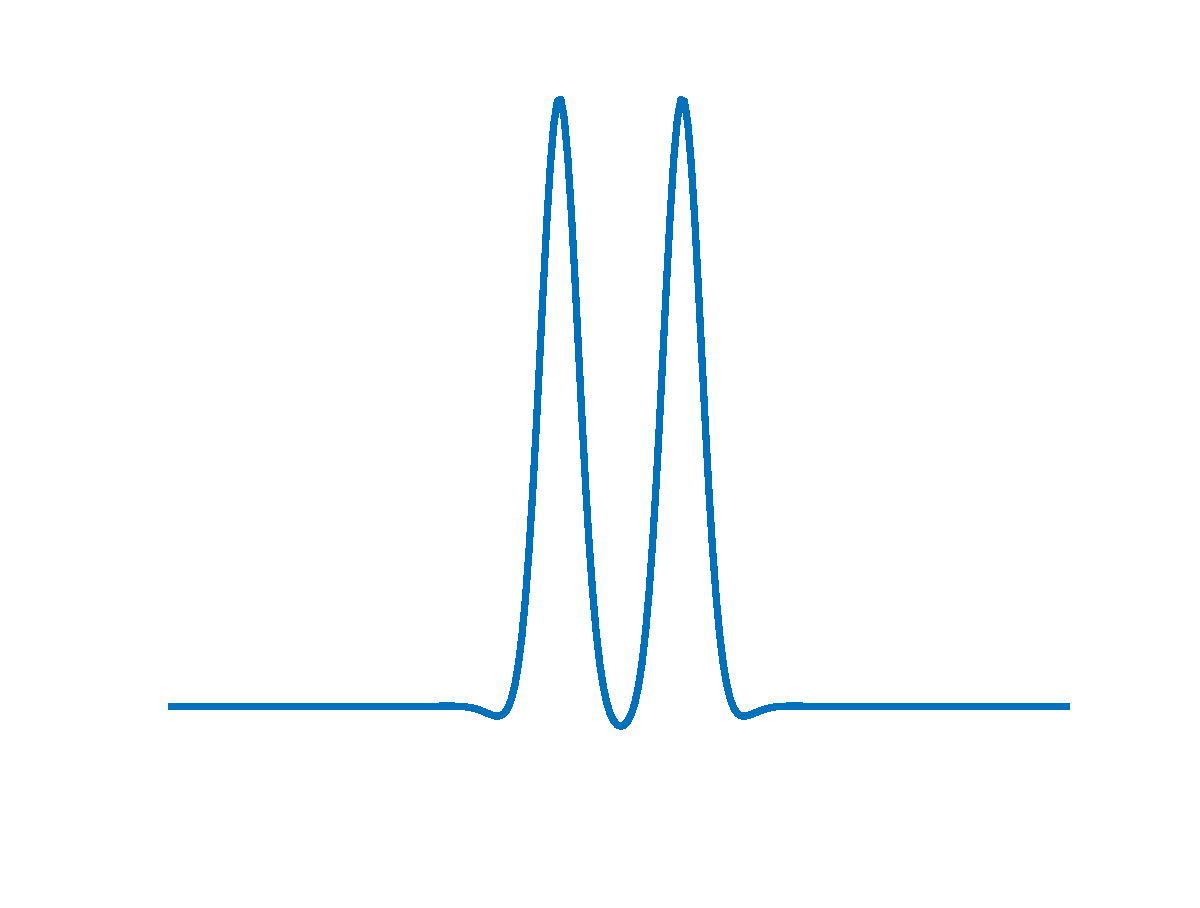
\includegraphics[width=4cm]{images/2pulseunstable}
		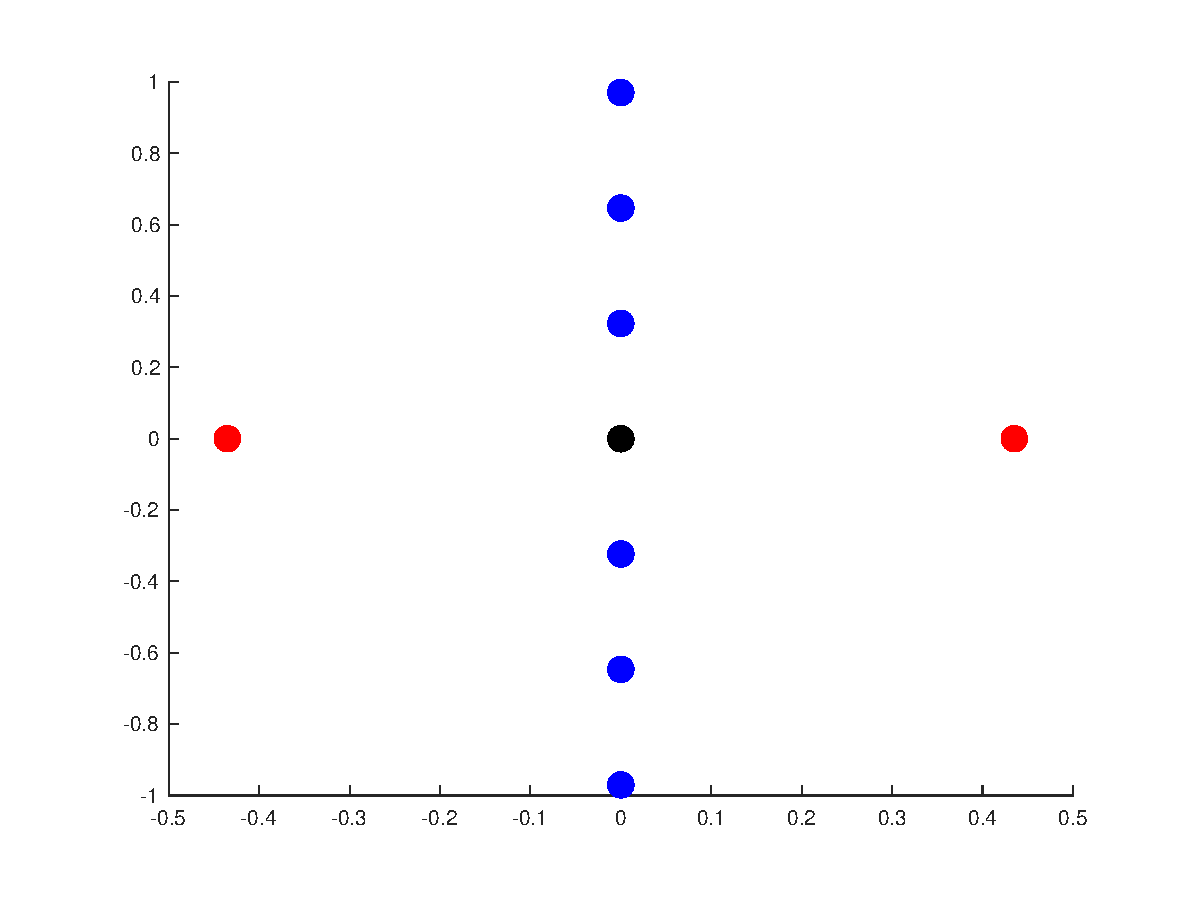
\includegraphics[width=4cm]{images/2pulseunstableeig}
		\end{center}
		\caption{\textcolor{red}{Interaction} eigenvalues and \textcolor{blue}{``essential spectrum''} eigenvalues for neutrally stable and unstable 2-periodic pulse.}
		\end{figure}
\end{frame}

\begin{frame}
	\frametitle{Krein bubbles}
	\fontsize{16}{7.2}\selectfont
	What happens when the period $X$ increases?
	\begin{itemize}
		\item Interaction eigenvalues are (roughly) constant
		\vspace{0.5cm}
		\item Essential spectrum eigenvalues
		\begin{align*}
    	\lambda_m^{\text{ess}}(r) &\approx c \frac{m \pi i}{X} && m \text{ nonzero integer}
    	\end{align*}
    	move towards the origin
		\vspace{0.5cm}
		\item Essential spectrum eigenvalue (positive Krein signature) will collide with interaction eigenvalue (negative Krein signature)
		\item Generically, this will cause the eigenvalues to move off of the imaginary axis
	\end{itemize}
\end{frame}

\begin{frame}
	\frametitle{Krein bubbles}
	\fontsize{16}{7.2}\selectfont
	\begin{center}
		\includemedia[
		     width=8cm,height=6cm,
		     activate=pageopen,
		     addresource=videos/Kreincollision.mp4,
		     flashvars={
		         source=videos/Kreincollision.mp4
		        &autoPlay=false
		     }
		]{}{VPlayer.swf} 
	\end{center}
\end{frame}

\begin{frame}
	\frametitle{Krein bubbles}
	\fontsize{16}{7.2}\selectfont
	Real and imaginary parts of eigenvalues near Krein bubble (numerical results from AUTO)
		\begin{figure}
		\begin{center}
		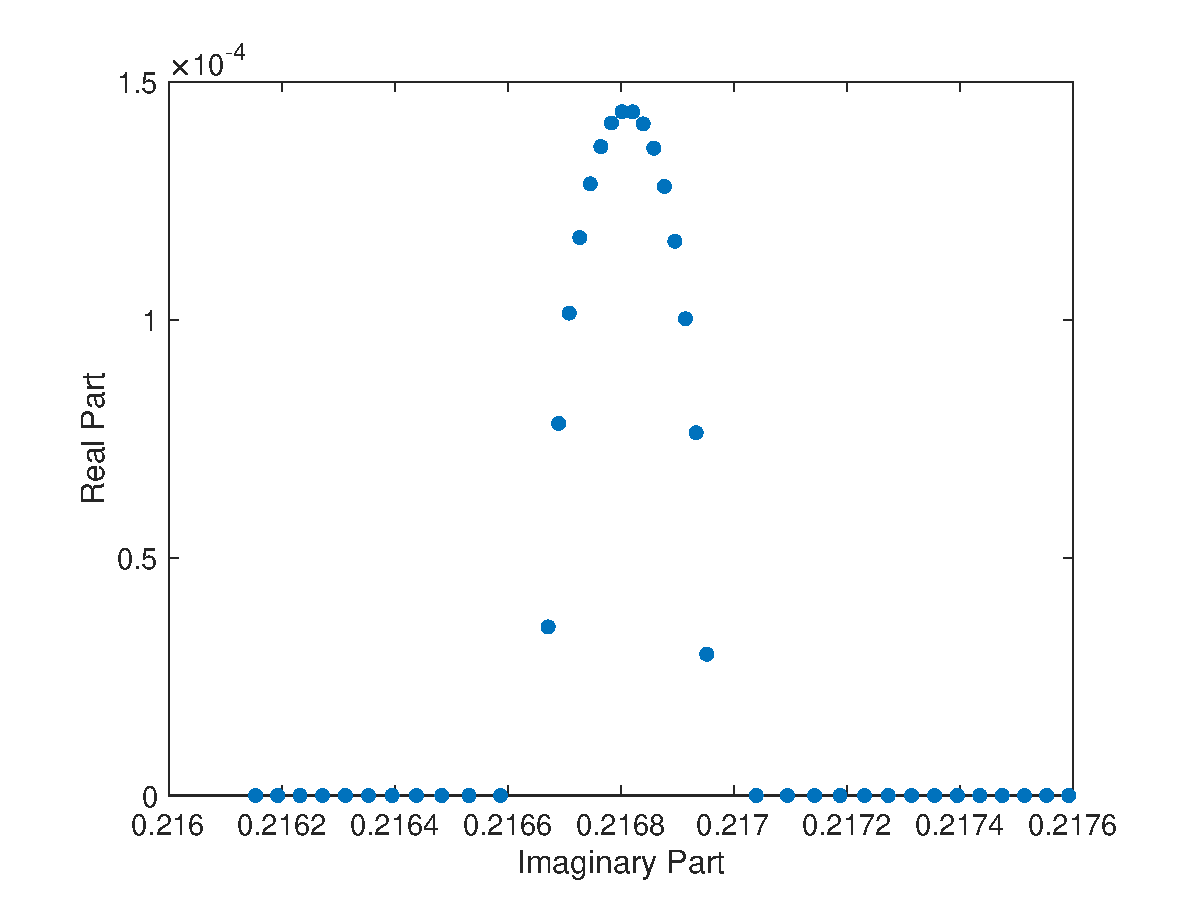
\includegraphics[width=8cm]{images/Kreinbubble1.eps}
		\end{center}
		\end{figure}
\end{frame}

\begin{frame}
	\frametitle{Krein bubbles}
	\fontsize{16}{7.2}\selectfont
	\begin{itemize}
		\item Brief instability bubble forms when eigenvalues collide on imaginary axis.
		\vspace{0.25cm}
		\item So far, only have numerical results.
		\vspace{0.25cm}
		\item A proof of this result should involve the off-diagonal terms in the block matrix.
		\vspace{0.25cm}
		\item The Krein bubble radius is smaller than the remainder terms in the block matrix equation.
		\vspace{0.25cm}
		\item A proof using this method is not possible without characterizing the higher order terms.
	\end{itemize}

\end{frame}

\section{Time stepping for 2-pulses}

\begin{frame}
	\frametitle{Time stepping}
	\fontsize{16}{7.2}\selectfont
	\begin{itemize}
		\item Suppose 2-pulse eigenvalue pattern on real line is 
		\begin{figure}
		\begin{center}
		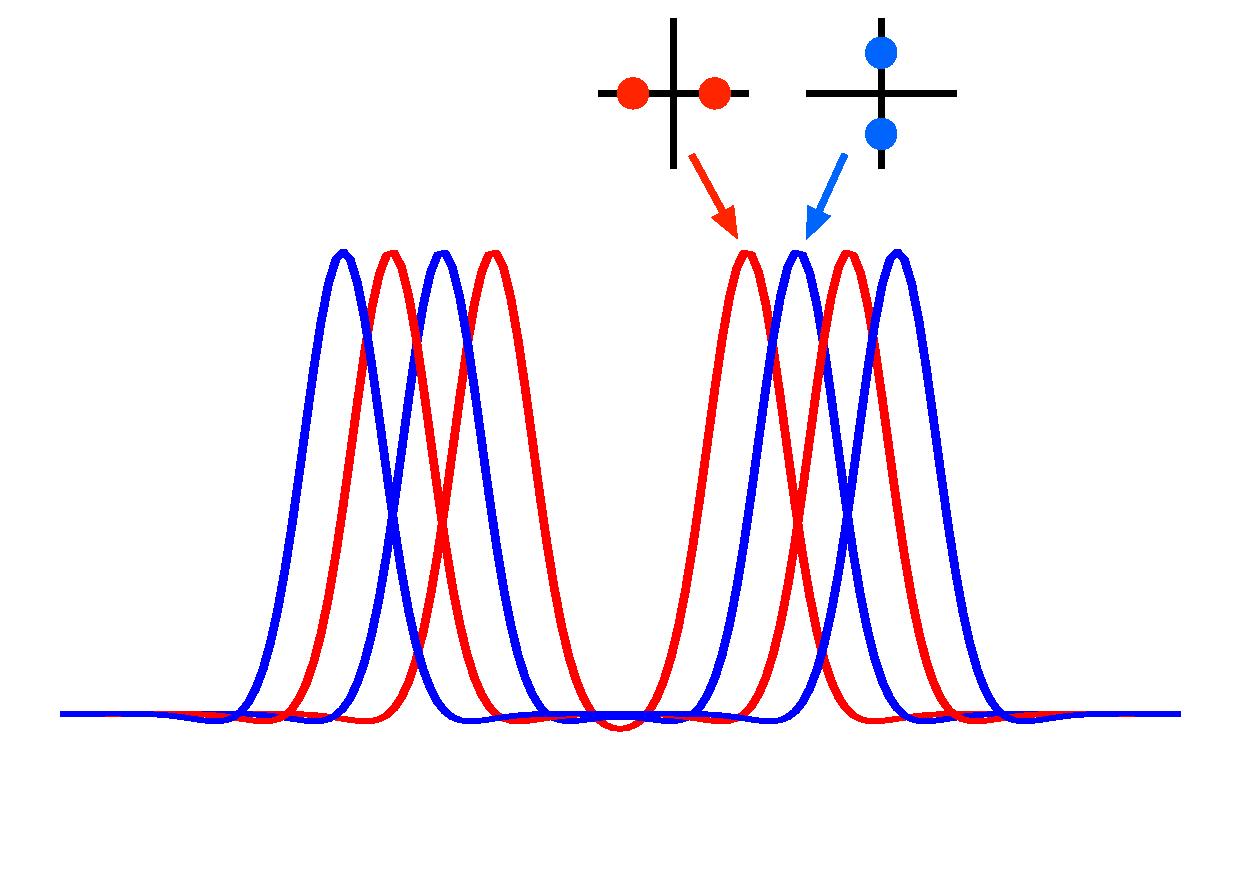
\includegraphics[width=5cm]{images/DPeigpattern.eps}
		\end{center}
		\end{figure}
		\item Numerics strongly suggests this is the case
		\vspace{0.5cm}
		\item What does this imply for PDE dynamics?
	\end{itemize}
\end{frame}

\begin{frame}
	\frametitle{Time stepping}
	\fontsize{16}{7.2}\selectfont
	\begin{itemize}
		\item What happens near the 2-pulse equilibria?
		\vspace{0.5cm}
		\item Time-stepping scheme:
		\begin{itemize}
			\item Chebyshev polynomial spectral discretization in space
			\item Dirichlet/Neumann boundary conditions
			\item Crank-Nicolson/Adams-Bashforth 2 IMEX scheme for time-stepping
		\end{itemize}
		\vspace{0.5cm}
		\item Initial condition: ``pull apart'' 2-pulses and let go!
	\end{itemize}
\end{frame}

\begin{frame}
	\frametitle{Time stepping, near unstable double pulse}
	\fontsize{16}{7.2}\selectfont
	\begin{center}
		\includemedia[
		     width=8cm,height=6cm,
		     activate=pageopen,
		     addresource=images/unstable.mp4,
		     flashvars={
		         source=images/unstable.mp4
		        &autoPlay=false
		     }
	]{}{VPlayer.swf} 
	\end{center}
\end{frame}

\begin{frame}
	\frametitle{Time stepping, near neutrally stable double pulse}
	\fontsize{16}{7.2}\selectfont
	\begin{center}
		\includemedia[
		     width=8cm,height=6cm,
		     activate=pageopen,
		     addresource=images/stable.mp4,
		     flashvars={
		         source=images/stable.mp4
		        &autoPlay=false
		     }
	]{}{VPlayer.swf} 
	\end{center}
\end{frame}

\begin{frame}
	\frametitle{Phase portrait}
	\fontsize{16}{7.2}\selectfont
	\begin{center}
	\includegraphics[width=0.8\linewidth]{images/phaseportrait2}
	\end{center}
\end{frame}

\begin{frame}
	\frametitle{Phase portrait}
	\fontsize{16}{7.2}\selectfont
	Resembles phase portrait of 2D ODE
	\begin{align*}
	\dot{x} &= y \\
	\dot{y} &= C e^{-\alpha x} \sin \beta x
	\end{align*}
	\begin{center}
	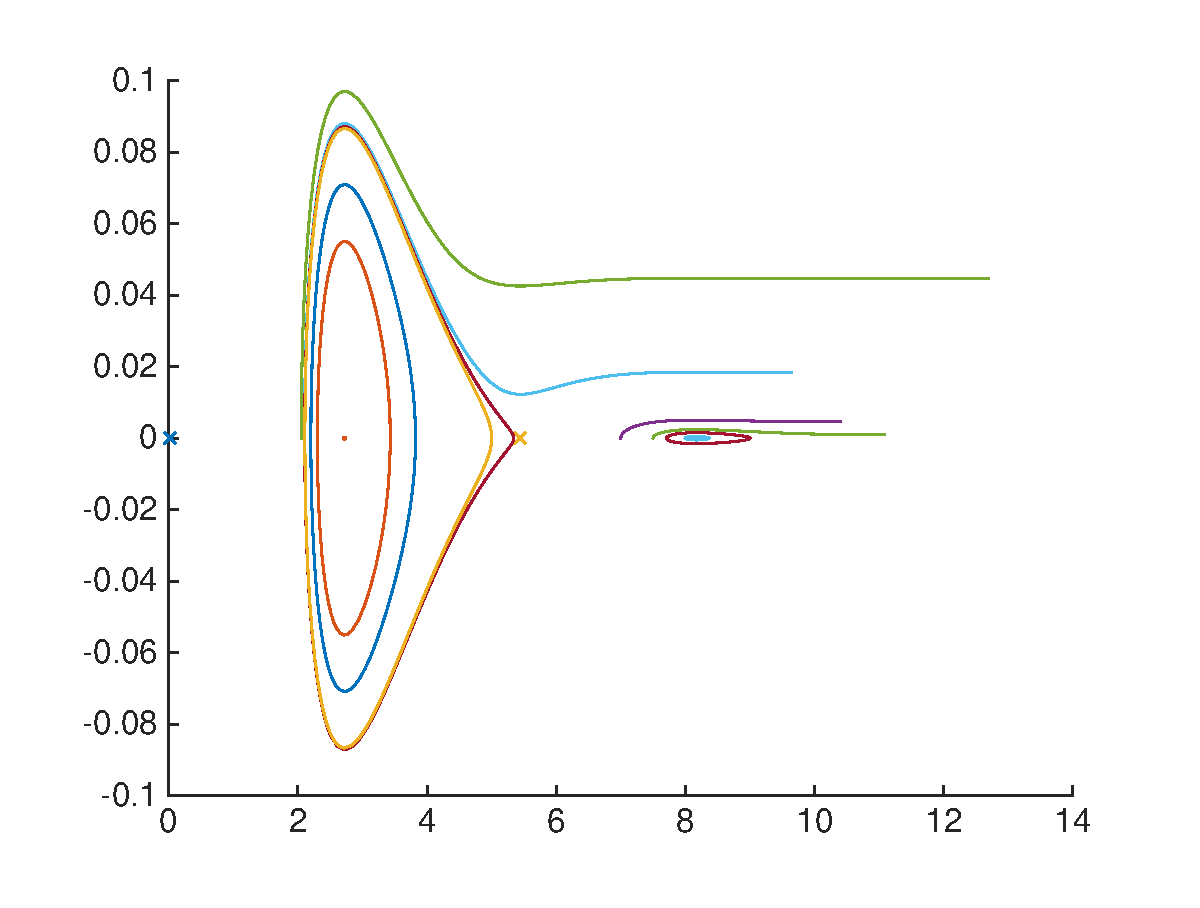
\includegraphics[width=0.5\linewidth]{images/simplephaseportrait}
	\end{center}
	Harmonic oscillator with spatially-varying restoring force
\end{frame}

\section{Multi-pulses in other systems}

\begin{frame}
	\frametitle{Chen-McKenna suspension bridge equation}
	\fontsize{16}{7.2}\selectfont
	\begin{itemize}
	\item Model for waves on suspended beam 
     \[ u_{tt} + u_{xxxx} + (u+1)^+ - 1 = 0 \]
     \begin{itemize}
     	\item $u$ is vertical displacement
     	\item Beam bends under its own weight
     	\item Restoring force is only for downward displacement
     \end{itemize}
     \item Smooth approximation
 	\[ u_{tt} + u_{xxxx} + e^{u} - 1 = 0 \]
 	 \item Equation has single and multi-pulse traveling wave solutions for wavespeeds $c \in (0, \sqrt{2})$.
 \end{itemize}
\end{frame}

\begin{frame}
\frametitle{Chen-McKenna: essential spectrum}
	\fontsize{16}{7.2}\selectfont
	Essential spectrum is purely imaginary and bounded from the origin.
	\[ \sigma_{ess} = [ (-\infty, r] \cup [r, \infty) ]i \]
	\begin{figure}
	\begin{center}
	\includegraphics[width=8cm]{images/essspeccombined.pdf}
	\end{center}
	\end{figure}
	Essential spectrum gap ``leaves room'' for imaginary interaction eigenvalues.
\end{frame}

\begin{frame}
\frametitle{Chen-McKenna: spectrum of multi-pulses}
	\fontsize{16}{7.2}\selectfont
\begin{figure}[H]
\begin{center}
\begin{tabular}{cc}
\includegraphics[width=0.2\textwidth]{images/chendouble1} & \includegraphics[width=0.2\textwidth]{images/chenspecdouble1} \\
\includegraphics[width=0.2\textwidth]{images/chendouble2} & \includegraphics[width=0.2\textwidth]{images/chenspecdouble2} \\
\end{tabular}
\end{center}
$k$ odd (top), $k$ even (bottom)
\end{figure}
\end{frame}

\begin{frame}
\frametitle{Discrete nonlinear Schr{\"o}dinger equation (DNLS)}
\fontsize{16}{7.2}\selectfont
\begin{equation*}
i\dot{\psi}_n + d(\psi_{n+1} - 2 \psi_n + \psi_{n-1}) + |\psi_n|^2 \psi_n = 0
\end{equation*}
\begin{itemize}
	\item Discrete analogue to nonlinear Schr{\"o}dinger equation 
	\item Parameter $d$ is strength of coupling between adjacent lattice sites in integer lattice
	\item Rotating wave solutions of form $\psi_n(t) = e^{i \omega t}\phi_n$
\end{itemize}
\end{frame}

\begin{frame}
\frametitle{DNLS: spectrum of multi-pulses}
\fontsize{16}{7.2}\selectfont
Interaction eigenvalue pattern determined by geometry of multi-pulse.
\begin{figure}[H]
\centering
\includegraphics[width=4.5cm]{images/dnlsPP.eps}
\includegraphics[width=4.5cm]{images/dnlsPPeig.eps}
\includegraphics[width=4.5cm]{images/dnlsPM.eps}
\includegraphics[width=4.5cm]{images/dnlsPMeig.eps}
\end{figure}
\end{frame}

\section{Future directions}

\begin{frame}
	\frametitle{Future directions}
	\fontsize{16}{7.2}\selectfont
	\begin{itemize}
		\item Characterize higher order terms in block matrix to see if this can be used to prove Krein bubble occurs.
		\vspace{0.5cm}
		\item Consider other approaches to spectral problem for periodic multi-pulses in Hamiltonian systems which might be more conducive to locating Krein bubble.
		\vspace{0.5cm}
		\item Time-stepping for double pulses in Krein bubble. What does the instability bubble imply for the evolution of the PDE.
		\vspace{0.5cm}
		\item Are any of the neutrally stable multi-pulses in KdV5, Chen-McKenna, or DNLS nonlinearly stable?
	\end{itemize}
\end{frame}

\begin{frame}
	\frametitle{References}
	\fontsize{12}{7.2}\selectfont
	\begin{enumerate}
		\item Buffoni B and S\'er\'e E. \emph{A global condition for quasi-random behaviour in a class of conservative systems}. Commun. Pure Appl. Math., 49 (1996), 285-305.
		\item Chugunova M and Pelinovsky P. \emph{Two-pulse solutions in the fifth-order KdV equation: Rigorous theory and numerical approximations}. Discrete and Continuous Dynamical Systems, Series B 8.4 (2007), 773-800.
		\item Groves M D. \emph{Solitary-wave solutions to a class of fifth-order model equations}. Nonlinearity, 11 (1998), 341-353.
		\item Sandstede B. \emph{Verzweigungstheorie homokliner Verdopplungen}. Ph.D. thesis, University of Stuttgart, 1993.
		\item Sandstede B. \emph{Stability of multiple-pulse solutions}. Trans. Am. Math. Soc., 350 (1998), 429-472.
		\item Sandstede B. \emph{Stability of travelling waves}. In: \emph{Handbook of Dynamical Systems II} (B Fiedler, ed). Elsevier (2002) 983-1055.
	\end{enumerate}
\end{frame}
 
\end{document}